\documentclass[11pt]{report}
\usepackage[utf8]{inputenc}
\usepackage{graphicx}
\usepackage{amsmath}
\usepackage{booktabs}
\usepackage{longtable}
\usepackage{float}
\usepackage[a4paper, top=2.5cm, bottom=2.5cm, left=2.5cm, right=2.5cm]{geometry}

\title{
    \vspace{2cm}
    \textbf{Machine Learning 441: Assignment 1} \\
    \large Data Exploration
}
\author{
    Ruan Buhr \\ 
    \small 26440873
}
\date{\today}

\begin{document}

\maketitle

\section*{Task 1: Data Quality Reports}

The \texttt{badDataSet.csv} data set contains 581012 instances, with 62 descriptive features and a single response.

\begin{table}[H]
\centering
\caption{Data Quality Report for the Descriptive Features.}
\label{tab:data_quality_report_des_feat}
\resizebox{\textwidth}{!}{
    \begin{tabular}{lrrrrrrrrrr}
\toprule
Feature & Count & \% Miss. & Card. & Min. & 1st Qrt. & Mean & Median & 3rd Qrt. & Max. & Std. Dev. \\
\midrule
A1 & 581012 & 0.00 & 1978 & 2054845.65 & 3104928.15 & 3271134.43 & 3311628.60 & 3496222.05 & 4264440.30 & 309481.13 \\
A2 & 578069 & 0.51 & 361 & 0.00 & 58.00 & 155.66 & 127.00 & 260.00 & 360.00 & 111.91 \\
A3 & 581012 & 0.00 & 576099 & 0.00 & 145.49 & 389.92 & 318.12 & 652.53 & 903.48 & 280.34 \\
A4 & 580708 & 0.05 & 67 & 0.00 & 9.00 & 14.10 & 13.00 & 18.00 & 66.00 & 7.49 \\
A5 & 578069 & 0.51 & 569 & -691.00 & 108.00 & 269.42 & 218.00 & 384.00 & 1397.00 & 212.56 \\
A6 & 581012 & 0.00 & 581012 & -173.07 & 6.99 & 46.42 & 29.91 & 68.97 & 600.95 & 58.30 \\
A7 & 578069 & 0.51 & 577988 & -1.00 & -0.50 & -0.00 & -0.00 & 0.50 & 1.00 & 0.58 \\
A8 & 581012 & 0.00 & 5811 & 0.00 & 1106.00 & 8158.11 & 1997.00 & 3328.00 & 510165098.00 & 1185156.02 \\
A9 & 578069 & 0.51 & 207 & 0.00 & 198.00 & 212.14 & 218.00 & 231.00 & 254.00 & 26.77 \\
A10 & 578069 & 0.51 & 186 & 0.00 & 213.00 & 223.32 & 226.00 & 237.00 & 254.00 & 19.77 \\
A11 & 581012 & 0.00 & 255 & 0.00 & 119.00 & 142.53 & 143.00 & 168.00 & 254.00 & 38.27 \\
A12 & 578069 & 0.51 & 5826 & 0.00 & 1024.00 & 1980.43 & 1710.00 & 2550.00 & 7173.00 & 1324.25 \\
A13 & 578069 & 0.51 & 2 & 0.00 & 0.00 & 0.45 & 0.00 & 1.00 & 1.00 & 0.50 \\
A14 & 581012 & 0.00 & 2 & 0.00 & 0.00 & 0.05 & 0.00 & 0.00 & 1.00 & 0.22 \\
A15 & 581012 & 0.00 & 2 & 0.00 & 0.00 & 0.44 & 0.00 & 1.00 & 1.00 & 0.50 \\
A16 & 578069 & 0.51 & 1 & 0.00 & 0.00 & 0.00 & 0.00 & 0.00 & 0.00 & 0.00 \\
A17 & 581012 & 0.00 & 1 & 0.00 & 0.00 & 0.00 & 0.00 & 0.00 & 0.00 & 0.00 \\
A18 & 578069 & 0.51 & 3 & 0.00 & 0.00 & 0.07 & 0.00 & 0.00 & 2.00 & 0.28 \\
A19 & 581012 & 0.00 & 2 & 0.00 & 0.00 & 0.50 & 0.00 & 1.00 & 1.00 & 0.50 \\
A20 & 577566 & 0.59 & 2 & 0.00 & 0.00 & 0.01 & 0.00 & 0.00 & 1.00 & 0.07 \\
A21 & 173355 & 70.16 & 2 & 0.00 & 0.00 & 0.01 & 0.00 & 0.00 & 1.00 & 0.07 \\
A22 & 581012 & 0.00 & 2 & 0.00 & 0.00 & 0.01 & 0.00 & 0.00 & 1.00 & 0.11 \\
A23 & 581012 & 0.00 & 2 & 0.00 & 0.00 & 0.01 & 0.00 & 0.00 & 1.00 & 0.09 \\
A24 & 581012 & 0.00 & 2 & 0.00 & 0.00 & 0.02 & 0.00 & 0.00 & 1.00 & 0.14 \\
A25 & 581012 & 0.00 & 2 & 0.00 & 0.00 & 0.00 & 0.00 & 0.00 & 1.00 & 0.05 \\
A26 & 581012 & 0.00 & 2 & 0.00 & 0.00 & 0.01 & 0.00 & 0.00 & 1.00 & 0.11 \\
A27 & 581012 & 0.00 & 2 & 0.00 & 0.00 & 0.00 & 0.00 & 0.00 & 1.00 & 0.01 \\
A28 & 581012 & 0.00 & 2 & 0.00 & 0.00 & 0.00 & 0.00 & 0.00 & 1.00 & 0.02 \\
A29 & 581012 & 0.00 & 2 & 0.00 & 0.00 & 0.00 & 0.00 & 0.00 & 1.00 & 0.04 \\
A30 & 581012 & 0.00 & 2 & 0.00 & 0.00 & 0.06 & 0.00 & 0.00 & 1.00 & 0.23 \\
A31 & 581012 & 0.00 & 2 & 0.00 & 0.00 & 0.02 & 0.00 & 0.00 & 1.00 & 0.14 \\
A32 & 581012 & 0.00 & 2 & 0.00 & 0.00 & 0.05 & 0.00 & 0.00 & 1.00 & 0.22 \\
A33 & 581012 & 0.00 & 2 & 0.00 & 0.00 & 0.03 & 0.00 & 0.00 & 1.00 & 0.17 \\
A34 & 581012 & 0.00 & 2 & 0.00 & 0.00 & 0.00 & 0.00 & 0.00 & 1.00 & 0.03 \\
A35 & 581012 & 0.00 & 2 & 0.00 & 0.00 & 0.00 & 0.00 & 0.00 & 1.00 & 0.00 \\
A36 & 581012 & 0.00 & 2 & 0.00 & 0.00 & 0.00 & 0.00 & 0.00 & 1.00 & 0.07 \\
A37 & 581012 & 0.00 & 2 & 0.00 & 0.00 & 0.01 & 0.00 & 0.00 & 1.00 & 0.08 \\
A38 & 581012 & 0.00 & 2 & 0.00 & 0.00 & 0.00 & 0.00 & 0.00 & 1.00 & 0.06 \\
A39 & 581012 & 0.00 & 2 & 0.00 & 0.00 & 0.01 & 0.00 & 0.00 & 1.00 & 0.08 \\
A40 & 581012 & 0.00 & 2 & 0.00 & 0.00 & 0.02 & 0.00 & 0.00 & 1.00 & 0.13 \\
A41 & 581012 & 0.00 & 2 & 0.00 & 0.00 & 0.00 & 0.00 & 0.00 & 1.00 & 0.04 \\
A42 & 581012 & 0.00 & 2 & 0.00 & 0.00 & 0.06 & 0.00 & 0.00 & 1.00 & 0.23 \\
A43 & 581012 & 0.00 & 2 & 0.00 & 0.00 & 0.10 & 0.00 & 0.00 & 1.00 & 0.30 \\
A44 & 581012 & 0.00 & 2 & 0.00 & 0.00 & 0.04 & 0.00 & 0.00 & 1.00 & 0.19 \\
A45 & 581012 & 0.00 & 2 & 0.00 & 0.00 & 0.00 & 0.00 & 0.00 & 1.00 & 0.03 \\
A46 & 581012 & 0.00 & 2 & 0.00 & 0.00 & 0.00 & 0.00 & 0.00 & 1.00 & 0.07 \\
A47 & 581012 & 0.00 & 2 & 0.00 & 0.00 & 0.00 & 0.00 & 0.00 & 1.00 & 0.04 \\
A48 & 581012 & 0.00 & 2 & 0.00 & 0.00 & 0.00 & 0.00 & 0.00 & 1.00 & 0.04 \\
A49 & 581012 & 0.00 & 2 & 0.00 & 0.00 & 0.20 & 0.00 & 0.00 & 1.00 & 0.40 \\
A50 & 581012 & 0.00 & 2 & 0.00 & 0.00 & 0.05 & 0.00 & 0.00 & 1.00 & 0.22 \\
A51 & 581012 & 0.00 & 2 & 0.00 & 0.00 & 0.04 & 0.00 & 0.00 & 1.00 & 0.21 \\
A52 & 581012 & 0.00 & 2 & 0.00 & 0.00 & 0.09 & 0.00 & 0.00 & 1.00 & 0.29 \\
A53 & 581012 & 0.00 & 2 & 0.00 & 0.00 & 0.08 & 0.00 & 0.00 & 1.00 & 0.27 \\
A54 & 581012 & 0.00 & 2 & 0.00 & 0.00 & 0.00 & 0.00 & 0.00 & 1.00 & 0.05 \\
A55 & 581012 & 0.00 & 2 & 0.00 & 0.00 & 0.00 & 0.00 & 0.00 & 1.00 & 0.06 \\
A56 & 581012 & 0.00 & 2 & 0.00 & 0.00 & 0.00 & 0.00 & 0.00 & 1.00 & 0.01 \\
A57 & 581012 & 0.00 & 2 & 0.00 & 0.00 & 0.00 & 0.00 & 0.00 & 1.00 & 0.02 \\
A58 & 581012 & 0.00 & 2 & 0.00 & 0.00 & 0.03 & 0.00 & 0.00 & 1.00 & 0.16 \\
A59 & 581012 & 0.00 & 2 & 0.00 & 0.00 & 0.02 & 0.00 & 0.00 & 1.00 & 0.15 \\
A60 & 581012 & 0.00 & 2 & 0.00 & 0.00 & 0.02 & 0.00 & 0.00 & 1.00 & 0.12 \\
A61 & 581012 & 0.00 & 581012 & 1.00 & 145253.75 & 290506.50 & 290506.50 & 435759.25 & 581012.00 & 167723.86 \\
A62 & 581012 & 0.00 & 1 & 1.00 & 1.00 & 1.00 & 1.00 & 1.00 & 1.00 & 0.00 \\
\bottomrule
\end{tabular}
}
\end{table}

Based on the data quality report in table~\ref{tab:data_quality_report_des_feat}, the 62 descriptive features exhibit highly varied characteristics,
from features with a significant percentage of missing values like A21 (70.16\%) to constant features with no variance like A17 and A62.

Task 2 and 3 will further analyze these findings and address the identified data quality issues.

\begin{table}[H]
\centering
\caption{Data Quality Report for the Response Feature.}
\label{tab:data_quality_report_res_feat}
\resizebox{\textwidth}{!}{
\begin{tabular}{lrrrrrrrrrr}
\toprule
Feature & Count & \% Miss. & Card. & Min. & 1st Qrt. & Mean & Median & 3rd Qrt. & Max. & Std. Dev. \\
\midrule
T & 580952 & 0.01 & 7 & 1.00 & 1.00 & 2.05 & 2.00 & 2.00 & 7.00 & 1.40 \\
\bottomrule
\end{tabular}
}
\end{table}

The data quality report for the response feature T, shown in table~\ref{tab:data_quality_report_res_feat}, indicates that it is an almost complete and discrete variable containing seven unique values
that are heavily skewed to toward the lower end of its range.


\section*{Task 2: Data Quality Issues}

\begin{longtable}{lp{4cm}p{7cm}}

\caption{Data Quality Issues.}
\label{tab:data_quality_issues} \\
\toprule
\textbf{Feature} & \textbf{Data Quality Issue} & \textbf{Justification} \\
\midrule
\endfirsthead

\caption[]{Data Quality Issues (continued).} \\
\toprule
\textbf{Feature} & \textbf{Data Quality Issue} & \textbf{Justification} \\
\midrule
\endhead

\multicolumn{3}{r}{\textit{Continued on next page}} \\
\endfoot

\bottomrule
\endlastfoot

A1 & Outliers & A1 has outliers on the lower and upper end of its distribution. The gap between the first quartile (3104928.15) and the minimum (2054845.65) is larger than the gap between the first quartile and the median (3311628.60). The gap between the maximum (4264440.30) and the third quartile (3496222.05) is also larger than the gap between the median and the third quartile. Figure~\ref{fig:a1_boxplot} confirms this finding.\\ 
\midrule
A2 & Systematic Missing Values &  A2 is missing 0.51\% of its values. It was found that features A2, A5, A7, A9, A10, A12, A13, A16, and A18 each have missing values when at least one of them do. To confirm that these missing values are co-located, programmatic analysis was done to count the number of observations containing a missing value in at least one of the features. This was then compared to the number of observations where all the features contained missing values. These two counts were both found to be 2943, 0.51\% of the 581012 observations. This provided definitive proof that the missing data are co-located. \\
\midrule
A3 & High Cardinality &  A3 contains 576099 unique values, which is very close to the number of instances. Figure~\ref{fig:correlation_with_T} shows that A3 exhibits a correlation of 0.017 with the response. This coupled with the fact that it has high cardinality means feature A3 probably provides minimal predictive power.  \\
\midrule
A3 & Perfect Positive Correlation with A2 & Figure~\ref{fig:A2_vs_A3_scatterplot} shows that A3 has a perfect positive linear correlation with A2. The correlation coefficient between A2 and A3 is exactly 1, supporting the findings in this scatterplot. \\
\midrule
A4 & Missing Values &  A4 is missing 0.05\% of its values. \\
\midrule
A4 & Outliers &  A4 has outliers in the upper range of its distribution. The gap between the maximum (66) and the third quartile (18) is larger than the gap between the median (13) and the third quartile. The boxplot in figure~\ref{fig:a4_boxplot} also shows that A4 has outliers in the upper range of its distribution. \\
\midrule
A5 & Systematic Missing Values &  A5 is missing 0.51\% of its values. Refer to table entry A2 for more detail. \\
\midrule
A5 & Outliers & A5 has outliers in the lower and upper ends of its distribution. Figure~\ref{fig:a5_boxplot} shows a boxplot that confirms the fact that A5 contains outliers. Figure~\ref{fig:a5_histplot} shows that A5 has a right-skewed distribution with the overwhelming majority of the values larger than zero. The fact that all negative values are also outliers suggests that they are data errors. \\
\midrule
A6 & High Cardinality & A6 contains 581012 unique values, which is exactly the number of instances in the dataset. Figure~\ref{fig:correlation_with_T} shows that A6 exhibits a correlation of 0.082 with the response. This coupled with the fact that it has extremely high cardinality means feature A6 provides minimal predictive power. \\
\midrule
A6 & Outliers & A6 has outliers in the lower and upper ends of its distribution. Figure~\ref{fig:a6_boxplot} shows a boxplot that confirms this. \\
\midrule
A7 & Systematic Missing Values & A7 is missing 0.51\% of its values.  Refer to table entry A2 for more detail. \\
\midrule
A7 & High Cardinality & A7 contains 577988 unique values, which is very close to the number of instances. Figure~\ref{fig:correlation_with_T} shows that A7 exhibits a correlation of 0 with the response. This coupled with the fact that it has high cardinality means feature A7 probably provides minimal predictive power. \\
\midrule
A7 & Uniform Distribution & Figure~\ref{fig:a7_histplot} shows the distribution of A7. It indicates that A7 has a uniform distribution over the range [-1, 1]. Since it has low correlation with the response and high cardinality it most likely provides no useful information. A7 is most likely just a uniformly generated random variable over the range [-1, 1]. \\
\midrule
A8 & Outliers & A8 contains a few extremely high value outliers in the upper end of its distribution. The maximum value of A8 is 510165098, which is much larger than the third quartile (3328). The boxplot in figure~\ref{fig:a8_boxplot} and the histogram in figure~\ref{fig:a8_histplot} both indicate how these outliers greatly skew the distribution of A8 to the right. The fact that the outliers are so much larger than the rest of the recorded value strongly suggest that they are errors. \\
\midrule
A9 & Systematic Missing Values & A9 is missing 0.51\% of its values.  Refer to table entry A2 for more detail. \\
\midrule
A9 & Outliers & A9 has outliers in the lower end of its distribution. Figure~\ref{fig:a9_boxplot} shows that A9 has a bunch of outliers in the lower end of its distribution. \\
\midrule
A10 & Invalid Values & The entries in A10 are all numeric except some entries that take on a value of \textit{a}. This creates a mixed-type feature that compromises data integrity. When loading the \texttt{badDataSet.csv} into a Pandas dataframe, all features are saved as integers or floats, except for A10. It is saved as an object since it contains integer values as well as \textit{a}. \\
\midrule
A10 & Systematic Missing Values & A10 is missing 0.51\% of its values.  Refer to table entry A2 for more detail. \\
\midrule
A10 & Outliers & Figure~\ref{fig:a10_boxplot} shows that A10 has numerous outliers in the lower range of its distribution. \\
\midrule
A11 & Outliers & Figure~\ref{fig:a11_boxplot} shows that A11 contains a bunch of outliers in the lower and upper ends of its distribution. \\
\midrule
A12 & Systematic Missing Values & A12 is missing 0.51\% of its values.  Refer to table entry A2 for more detail. \\
\midrule
A12 & Outliers & Figure~\ref{fig:a12_boxplot} shows that A12 contains a bunch of outliers in the upper end of its distribution. \\
\midrule
A13-A15, \& A19-A60 & Binary Cardinality & These features all have a cardinality of two. A13-A15 \& A19-A60 are two separate groups of one-hot encoding features of original categorical features. The heatmap in figure~\ref{fig:binary_heatmap} clearly shows two distinct regions where the entries are negatively correlated with one another. This is a strong suggestion that the two groups represent binary one-hot encoded features of original categorical features. \\
\midrule
A13 & Systematic Missing Values & A13 is missing 0.51\% of its values.  Refer to table entry A2 for more detail. \\
\midrule
A16 & Systematic Missing Values & A16 is missing 0.51\% of its values.  Refer to table entry A2 for more detail. \\
\midrule
A16 & Low Cardinality & A16 has a cardinality of one. All instances of A16 take on a value of 0. This means A16 is a constant value and provides no predictive power, since the value never changes. \\
\midrule
A17 & Low Cardinality & A17 has a cardinality of one. All instances of A17 take on a value of 0. Just like A16, this means that A17 provides no predictive power since it is a constant feature. \\ 
\midrule
A18 & Systematic Missing Values & A18 is missing 0.51\% of its values.  Refer to table entry A2 for more detail. \\
\midrule
A18 & Low Cardinality & A18 has a cardinality of three. All instances of A18 take on values of 0, 1, or 2 meaning that A18 likely represents a three-level categorical feature. \\
\midrule
A20 & Missing Values & A20 is missing 0.59\% of its values. \\
\midrule
A21 & Missing Values & A21 is missing 70.16\% of its values. This means that for over two thirds of the observations, there is no recorded value of A21. The vast majority of the feature is missing. \\
\midrule
A61 & High Cardinality & A61 contains 581012 unique values, which is exactly the same as the number of observations. A61 is most likely a unique identifier for each observation. The values range from 1 to 581012. The value of the first quartile is 145253.75. Pandas, which is a Python package to wrangle data, uses the following formula to calculate the position of the quartiles: $Position = 1 + \frac{k}{4} \times (N - 1)$. If one plugs the quantities $k = 1$ and $N = 581012$ then the calculated position for the first quartile is 145253.75, which is exactly the observed value of the 1st quartile of A61. The same holds for the median and the 3rd quartile. Also for any uniformly increasing sequence the average is the midpoint between the first and last numbers, this means if A61 is a uniformly increasing unique identifier for each row then the average should be $\frac{(1 + 581012)}{2} = 290506.5$, which is the value observed for the mean. The statistical properties of A61 perfectly match those of a simple uniformly increasing sequence from 1 to 581012. This clearly indicates that A61 is a unique identifier for each observation and does not have any predictive power. \\
\midrule
A62 & Low Cardinality & A62 has a cardinality of one. All instances of A62 take on a value of 1. This means A62 is a constant value and provides no predictive power, since the value never changes. \\
\midrule
T & Missing Values & T is missing 0.01\% of its values. \\
\end{longtable}

\section*{Task 3: Addressing The Data Quality Issues}

\begin{longtable}{p{2cm}p{3cm}p{4cm}p{6cm}}

\caption{Addressing Data Quality Issues.}
\label{tab:address_data_quality_issues} \\
\toprule
\textbf{Feature} & \textbf{Data Quality Issue} & \textbf{Handling Strategy} & \textbf{Justification} \\
\midrule
\endfirsthead

\caption[]{Addressing Data Quality Issues (continued).} \\
\toprule
\textbf{Feature} & \textbf{Data Quality Issue} & \textbf{Handling Strategy} & \textbf{Justification} \\
\midrule
\endhead

\multicolumn{4}{r}{\textit{Continued on next page}} \\
\endfoot

\bottomrule
\endlastfoot

A1 & Outliers & Keep outliers but mitigate their influence using a clamp transformation. & Figure~\ref{fig:a1_boxplot} shows that A1 has a lot of outliers on the upper and lower ends of its distribution. They appear as dense clusters outside the whiskers, suggesting they might be part of the natural tails of the distribution rather than data entry errors. Removing them would result in a loss of information and might harm a models performance. The best option to deal with the outliers present in A1 is to keep them and use a clamp transformation. A good approach is to set all values above the 99th percentile to the value of the 99th percentile, and the value below the 1st percentile to the 1st percentile. This doesn't discard any data, it simply reduces the influence of the most extreme values. \\
\midrule
A2 & Systematic Missing Values & Remove observations with missing values. & Features A2, A5, A7, A9, A10, A12, A13, A16, and A18 each have missing values when at least one of them do. To confirm that these missing values are co-located, programmatic analysis was done to count the number of observations containing a missing value in at least one of the features. This was then compared to the number of observations where all the features contained missing values. These two counts were both found to be 2943, 0.51\% of the 581012 observations. This provided definitive proof that the missing data occurs in the same observations. Since the 2943 observations are all missing a large portion of their data, and they make up a small percentage of all observations it is best to remove them from the dataset. \\
\midrule
A3 & High Cardinality & Remove A3 from the dataset. & A3 has a cardinality of 576099, which is very close to the number of observations, 581012. This coupled with the fact that A3 has a correlation of 0.017 with the response variable strongly suggests that A3 is a useless feature that will most likely just cause any model to overfit.\\
\midrule
A3 & Perfect Positive Correlation with A2 & Remove A3 from the dataset. & Figure~\ref{fig:A2_vs_A3_scatterplot} shows that A3 has a perfect positive correlation with A2. The line starts at (0, 0) which means that A3 is likely just a scaled version of A2. This means that including both A2 and A3 in the dataset is redundant and does not provide any new information. \\
\midrule
A4 & Missing Values & Impute missing values with the median of A4. & A4 is missing only 0.05\% of its values, which is not a lot. Imputing the missing values in this case will not introduce any bias in the dataset. Since A4 contains outliers in the upper range of its distribution it is better to impute the missing values of A4 with the median. \\
\midrule
A4 & Outliers & Transform A4 to reduce its skewness. & Figure~\ref{fig:a4_boxplot} shows that A4 has a right-skewed distribution with numerous outliers in the upper range of its distribution. These outliers form a natural part of the distribution of A4, and should not be removed as that will result in a loss of information. The best way to deal with outliers due to a skew distribution is to transform the feature to reduce skewness. By making A4 more symmetrical the influence of the outliers is reduced. Applying a $log(x+1)$ or a $sqrt(x)$ transformation are both valid approaches to reduce the skewness of A4. \\
\midrule
A5 & Systematic Missing Values & Remove observations with missing values. & Refer to table entry A2 for more detail. \\
\midrule
A5 & Outliers & Remove outliers in the lower end of the distribution and apply a transformation to reduce skewness to address the outliers in the upper end of the distribution of A5. & A5 has a few outliers in the lower end of its distribution below zero, since the overwhelming majority of the data is larger than zero, this is most likely a data entry error and it would be wise to remove these entries. After these entries have been removed, transform A5 the same as A4. This is because A5 also has a right-skew distribution and the outliers in the upper range of its distribution form part of the natural distribution of the data and removing them would result in a loss of information. \\
\midrule
A6 & High Cardinality & Remove A6 from the dataset. & A6 has a cardinality of 581012, which is exactly the number of observations in the dataset. This coupled with the fact that A6 has a correlation of 0.082 with the response variable strongly suggests that A6 is a useless feature that will most likely just cause any model to overfit. \\
\midrule
A6 & Outliers & Transform A6 to reduce its skewness. & Figure~\ref{fig:a6_boxplot} shows that A6 has an extreme right-skewed distribution, with the outliers in the upper and lower ends of the distribution forming part of the natural distribution of the data, the best way to handle these outliers and mitigate their influence it so apply a transformation to reduce the skewness of A6. This keeps all information while reducing the influence of the outliers. \\
\midrule
A7 & Systematic Missing Values & Remove observations with missing values. & Refer to table entry A2 for more detail. \\
\midrule
A7 & High Cardinality & Remove A7 from the dataset. & A7 has a cardinality of 577988, which is very close to the number of observation in the dataset. This coupled with the fact that A6 has a correlation of 0 with the response variable strongly suggests that A7 is a useless feature that will most likely just cause any model to overfit. \\
\midrule
A7 & Uniform Distribution & Remove A7 from the dataset & Figure~\ref{fig:a7_histplot} shows that A7 has an approximately uniform distribution over the range [-1, 1]. Since it has low correlation with the response and high cardinality A7 is most likely just a uniformly generated random variable over the range [-1, 1], and removing it from the dataset will not result in a loss of information. \\
\midrule
A8 & Outliers & Remove the outliers. & There is a huge difference between the outliers in the upper range of A8s distribution and the third quartile of A8. So much so that the distribution is extremely right-skewed. The fact that the distribution of A8 is this skewed and it contains a few outliers of extreme value strongly suggest that they are data errors and the best approach would be to remove them from the dataset. \\
\midrule
A9 & Systematic Missing Values & Remove observations with missing values. & Refer to table entry A2 for more detail. \\
\midrule
A9 & Outliers & Transform A9 to reduce its skewness. & Figure~\ref{fig:a9_boxplot} shows that A9 has a left-skewed distribution, with outliers in the lower end of its distribution. These values most likely form part of the natural distribution of the data and removing them will result in a loss of information. The best approach to deal with these outliers is to apply a logarithmic or a square root transformation to mitigate the influence of the outliers, while keeping all the information they represent. One thing to keep in mind is that since the data is left-skewed one cannot just simply apply the standard logarithmic or square root transformation, one first needs to reflect that data to make it right-skewed and then apply the transformation. \\
\midrule
A10 & Systematic Missing Values & Remove observations with missing values. & Refer to table entry A2 for more detail. \\
\midrule
A10 & Invalid Values & Treat invalid values as missing values and impute with median. & A10 entries are all numeric, except some entries that have a value of \textit{a}. To handle this the best strategy is to treat the entries with observed values \textit{a} as missing values and impute them with the median of A10. This is because A10 has outliers in the lower range of its distribution. \\
\midrule
A10 & Outliers & Transform A10 to reduce its skewness. &  Figure~\ref{fig:a10_boxplot} shows that A10 has a distribution extremely similar to that of A9. Both are left-skewed and would benefit from a transformation to reduce the influence of the outliers while keeping all the information they represent as they form a natural part of the distribution of these features. \\
\midrule
A11 & Outliers & Keep outliers, but mitigate their influence using a clamp transformation. & Figure~\ref{fig:a11_boxplot} shows that A11 has a roughly bell-shaped distribution. The outliers on both ends of the distribution appear to be part of the natural tails of the distribution rather than data errors. The best solution to mitigate the influence of these outliers is to use a clamp transformation, like setting all values above the 99th percentile to the 99th percentile, and all values below the first percentile to the first percentile. This reduces the influence of the most extreme outliers without changing the distribution of A11. \\
\midrule
A12 & Systematic Missing Values & Remove observations with missing values. & Refer to table entry A2 for more detail. \\
\midrule
A12 & Outliers & Transform A12 to reduce its skewness. & Figure~\ref{fig:a12_boxplot} shows that A12 has a right skewed distribution with outliers in the upper range of the distribution. These outliers appear to be part of the natural shape of the distribution and removing them would result in a loss of information. The best approach to handle this issue is to use a transformation like the logarithmic or square root transformation. This mitigates the influence of the outliers while preserving any information they represent. \\
\midrule
A13-A15, \& A19-A60 & Binary Cardinality & Treat these features as one-hot encoded features & As mentioned in table~\ref{tab:data_quality_report_res_feat} features A13-A15 \& A19-A60 form two distinct groups of one-hot encoded features of two distinct original categorical features. The A19-A60 is a one-hot encoding of a 42 level categorical variable and using this in certain machine learning contexts might lead to overfitting. Whether it is better to keep these variables one-hot encoded or revert back to the original categorical representation is completely dependent on the original values of the feature and the machine learning model to use. \\
\midrule
A13 & Systematic Missing Values & Remove observations with missing values. & Refer to table entry A2 for more detail. \\
\midrule
A16 & Systematic Missing Values & Remove observations with missing values. & Refer to table entry A2 for more detail. \\
\midrule
A16 & Low Cardinality & Remove A16 from the dataset. & A16 is a constant feature, all observations take on a value of 0. This means A16 is a constant feature and provides no predictive power. Including A16 in the dataset will lead to an increase in complexity without adding any information. \\
\midrule
A17 & Low Cardinality & Remove A17 from the dataset. & Just like A16, A17 is a constant feature, all observations also take on a value of 0. Including A17 in the dataset adds complexity without adding any new information. \\
\midrule
A18 & Systematic Missing Values & Remove observations with missing values. & Refer to table entry A2 for more detail. \\
\midrule
A18 & Low Cardinality & Treat A18 as a three-level categorical feature. & All instances of A18 take on values of 0, 1, or 2 meaning that A18 likely represents a hashed version of some original categorical feature. \\
\midrule
A20 & Missing Values & Impute with 0. & A20 has a cardinality of 2, and it is part of the A19-A60 one-hot encoded feature group. Because A20 is part of this large group of encoded features, its mean is 0.01 which means that 99\% of the non-missing values are 0. This overwhelming imbalance makes imputing the missing values with 0 the most logical choice. Further, imputing the missing 0.59\% of the values with 0 will have negligible impact on the feature's already skewed distribution. \\
\midrule
A21 & Missing Values & Remove A21 from the dataset. & Feature A21 is missing 70.16\%. This means the vast majority of the feature is missing. The best course of action is to remove the feature from the dataset, because A21 carries very little reliable information, and has low predictive power. Also imputing the missing values would fabricate 70.16\% of the values of the feature, which would introduce extreme bias in the feature, which will harm any models performance. \\
\midrule
A61 & High Cardinality & Remove A61 from the dataset. & A21 contains 581012 unique values, which is exactly the same as the number of observations in the dataset. As mentioned in table~\ref{tab:data_quality_report_res_feat}, A61 is almost certainly a unique identifier for each observation in the dataset and including it in the dataset will not provide any useful information about the response. \\
\midrule
A62 & Low Cardinality & Remove A62 from the dataset. & A62 is a constant feature, with all observations taking on a value of 1. This means it provides no information about the response and has no predictive power. Including A62 in the dataset will lead to an increase in complexity without adding any new information. \\
\midrule
T & Missing Values & Replace with mode. & T is known to be a seven-level categorical variable. It is only missing 0.01\% of its values, so imputing these values with the mode, which is 2, will not negatively impact the distribution of T. \\
\end{longtable}


\section*{Supporting Figures}

The following subsection contains figures and discussions that support the data quality issues mentioned in table~\ref{tab:data_quality_issues}.

\begin{figure}[H]
    \centering
    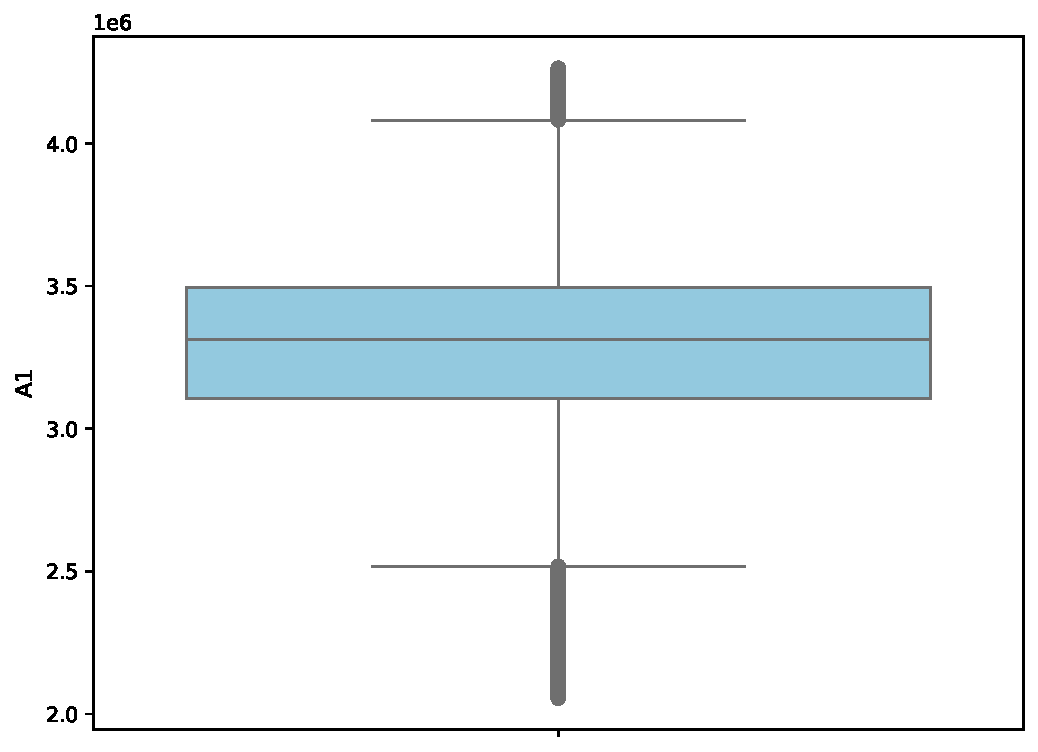
\includegraphics[width=0.6\textwidth]{images/A1_boxplot.pdf}
    \caption{Boxplot of A1.}
    \label{fig:a1_boxplot}
\end{figure}

\begin{figure}[H]
    \centering
    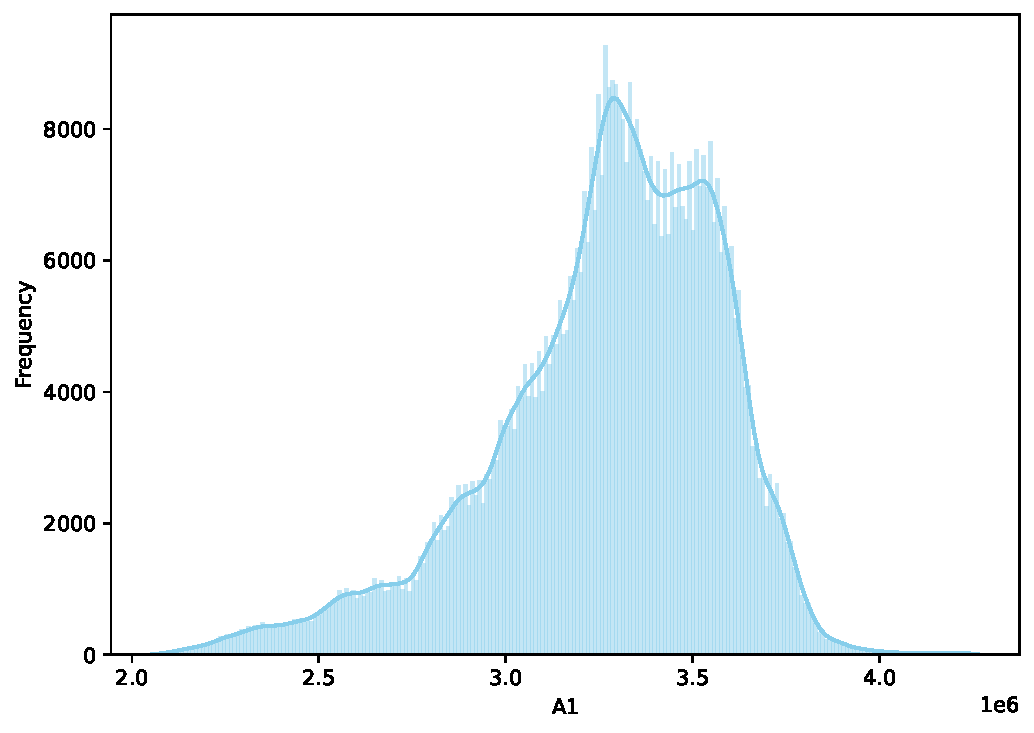
\includegraphics[width=0.6\textwidth]{images/A1_histplot.pdf}
    \caption{Histogram of A1.}
    \label{fig:a1_histplot}
\end{figure}

The boxplot in figure~\ref{fig:a1_boxplot} provides a visual confirmation of the outliers in feature A1. The central box represents the interquartile range (IQR), containing the middle 50\% of the data. The points extending far below and above the whiskers of the box are individual data points identified as outliers. This visualization clearly shows that a significant number of outliers exist at both the lower and upper ends of the distribution. Figure~\ref{fig:a1_histplot} shows that these outliers appear to be part of the natural distribution of A1 and removing them would lead to a loss of information. Since the data is not drastically skewed the best approach to mitigate the effect of these outliers on a model is to use a clamp transformation.

\begin{figure}[H]
    \centering
    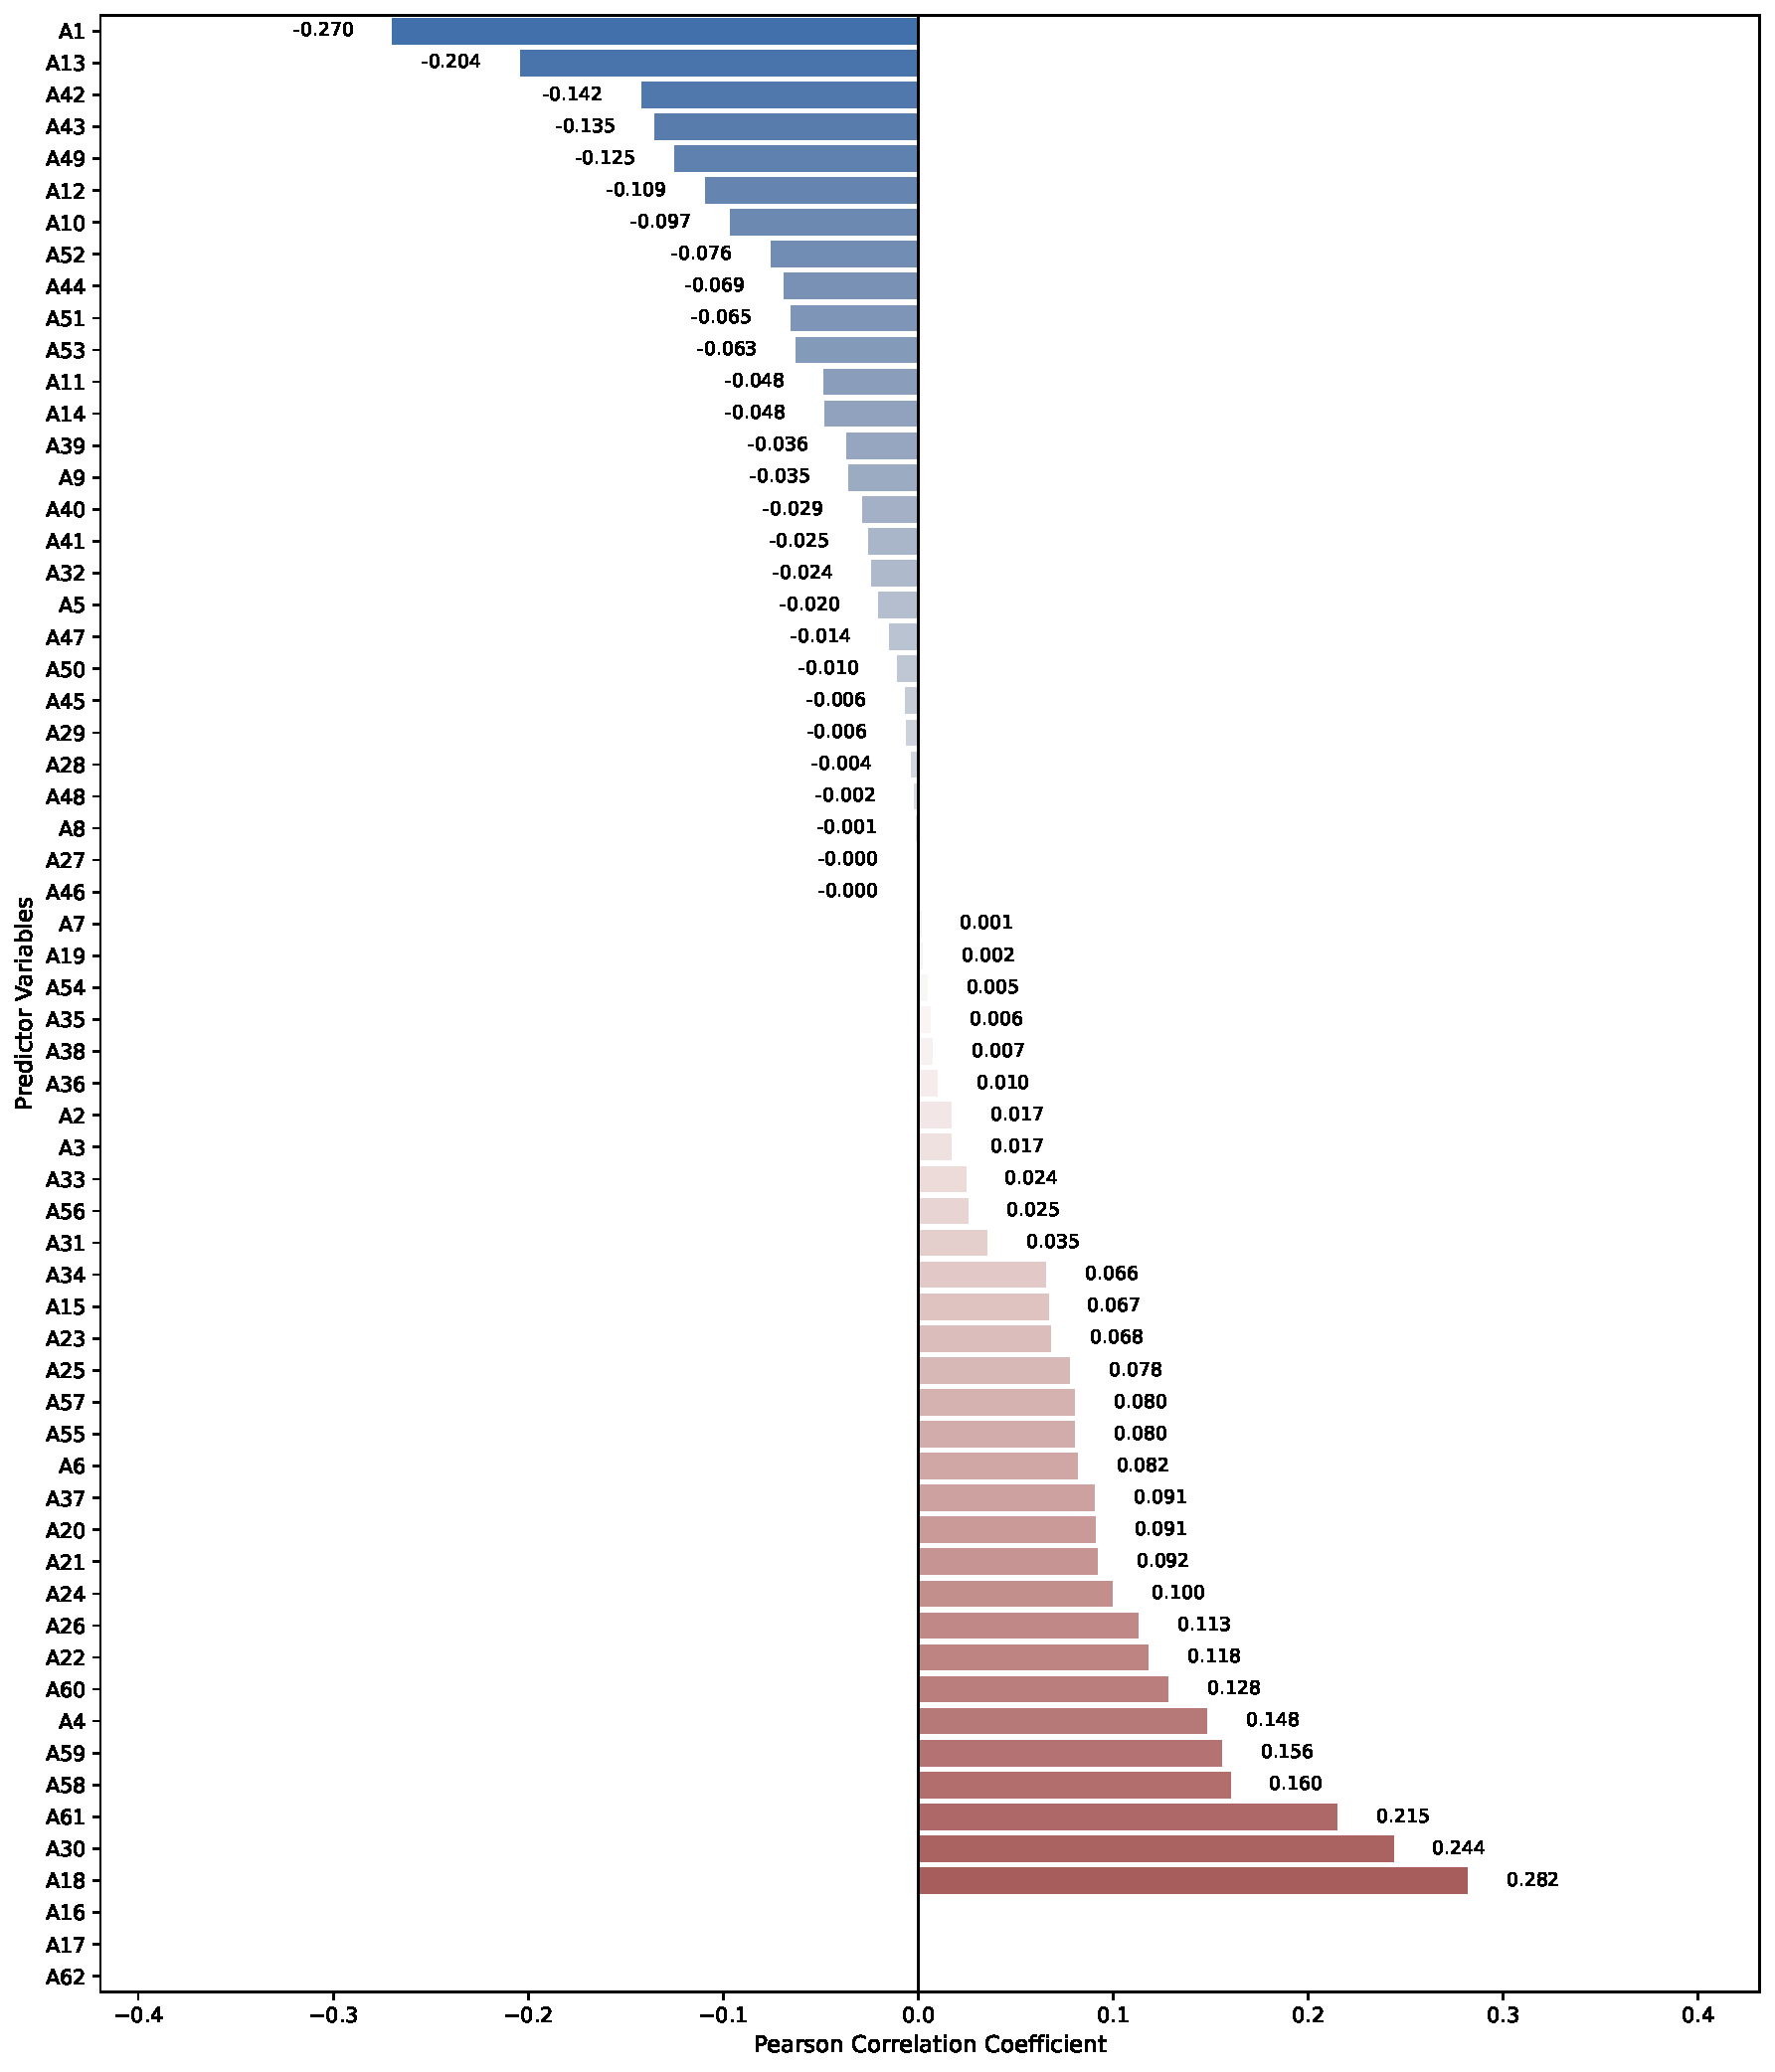
\includegraphics[width=0.6\textwidth]{images/correlation_with_T.pdf}
    \caption{Correlation of Each Predictor with Response Variable.}
    \label{fig:correlation_with_T}
\end{figure}

Figure~\ref{fig:correlation_with_T} illustrates the Pearson correlation coefficient, which measures the linear relationship between each predictor and the response. The analysis shows that most features have a weak to moderate correlation with the response, with all values falling between -0.27 and 0.29. This indicates that no single feature is a dominant predictor, suggesting that an effective model will need to leverage a combination of multiple features.

\begin{figure}[H]
    \centering
    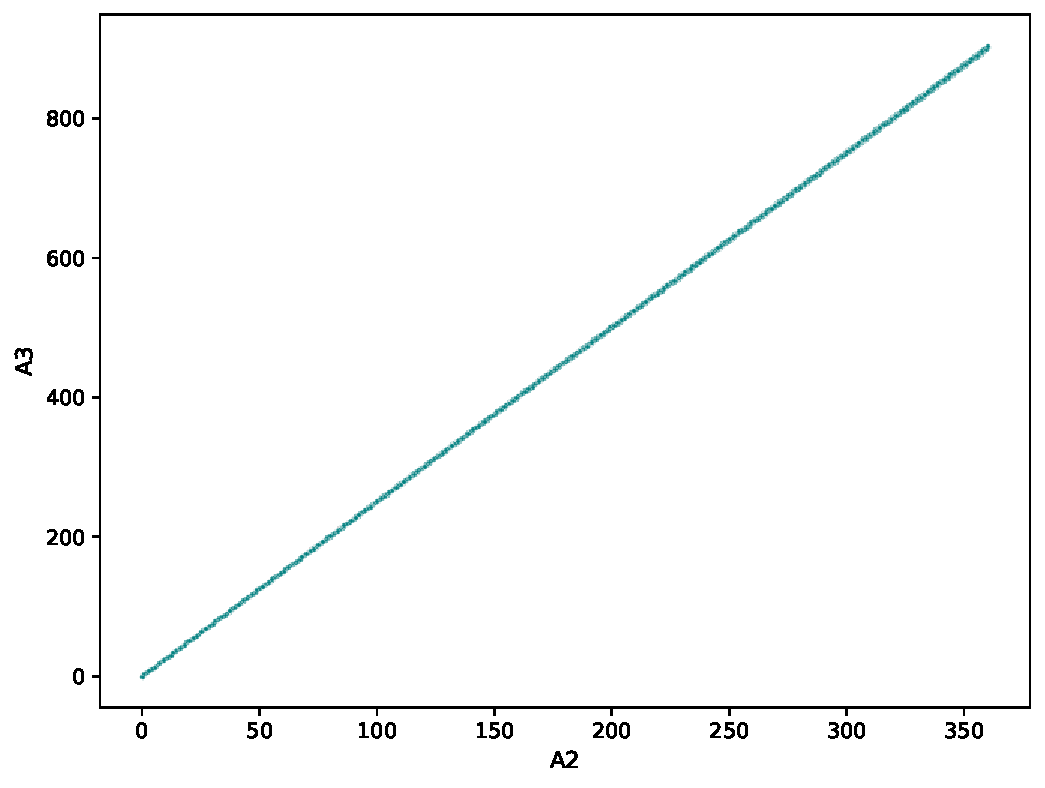
\includegraphics[width=0.6\textwidth]{images/A2_vs_A3_scatterplot.pdf}
    \caption{Scatterplot of A2 vs A3.}
    \label{fig:A2_vs_A3_scatterplot}
\end{figure}

Figure~\ref{fig:A2_vs_A3_scatterplot} shows that there is an extremely strong, positive, and linear relationship between A2 and A3. The line appears to start at the origin which indicates that A3 is just be a scaled version of A2. This means that the two variables are redundant and including both in the dataset does not provide any new information.

\begin{figure}[H]
    \centering
    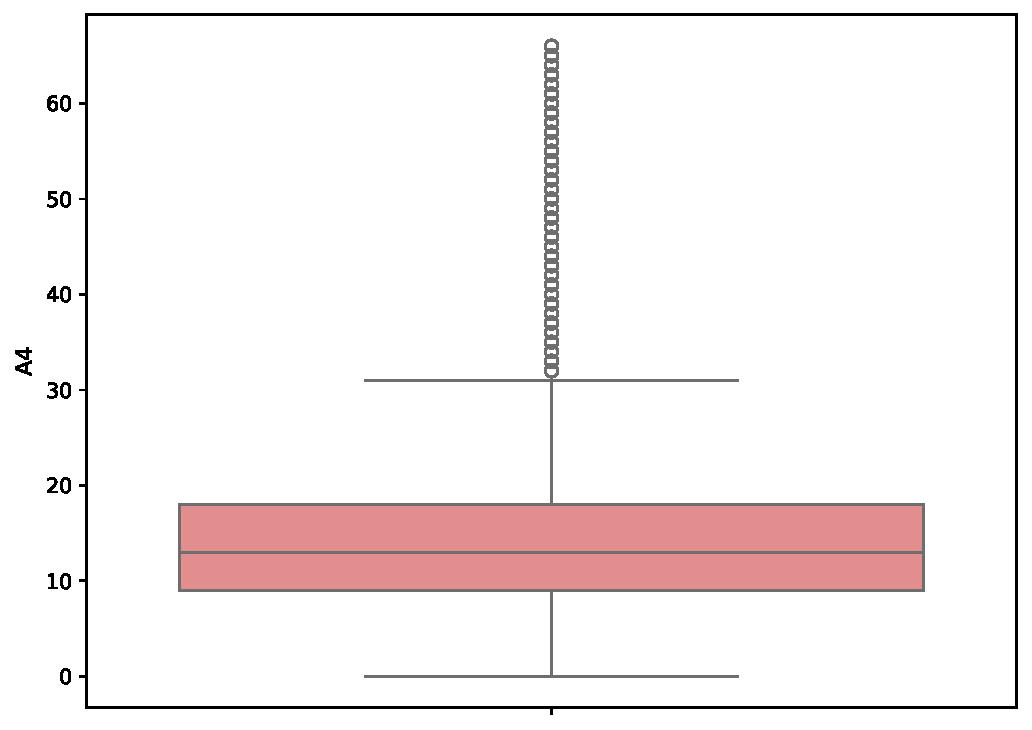
\includegraphics[width=0.6\textwidth]{images/A4_boxplot.pdf}
    \caption{Boxplot of A4.}
    \label{fig:a4_boxplot}
\end{figure}

\begin{figure}[H]
    \centering
    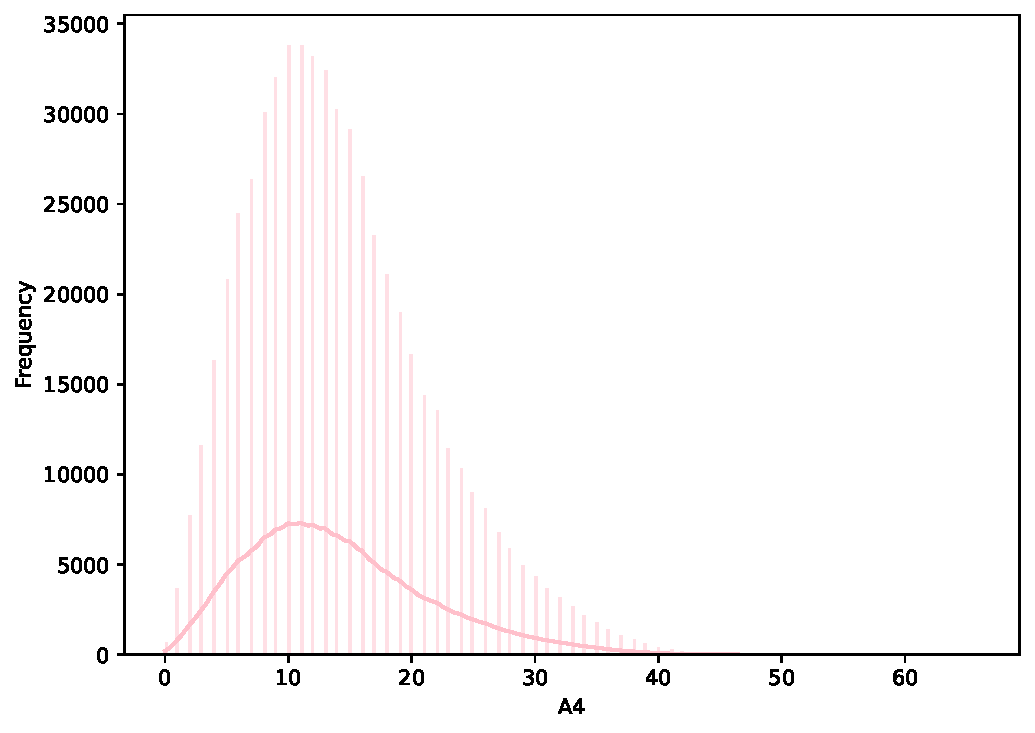
\includegraphics[width=0.6\textwidth]{images/A4_histplot.pdf}
    \caption{Histogram of A4.}
    \label{fig:a4_histplot}
\end{figure}

The boxplot in figure~\ref{fig:a4_boxplot} shows that A4 has outliers in the upper range of its distribution. The histogram in figure~\ref{fig:a4_histplot} show that these outliers appear to be part of the natural distribution of A4, as A4 appears to be right-skewed, and removing them would result in a loss of information. To mitigate the influence of these issues a transformation could be used to make A4 less skew, like a logarithmic transformation $log(x+1)$ or a square root transformation $sqrt(x)$. This keeps the information represented by the outliers, but reduces their effect on the fitted model.

\begin{figure}[H]
    \centering
    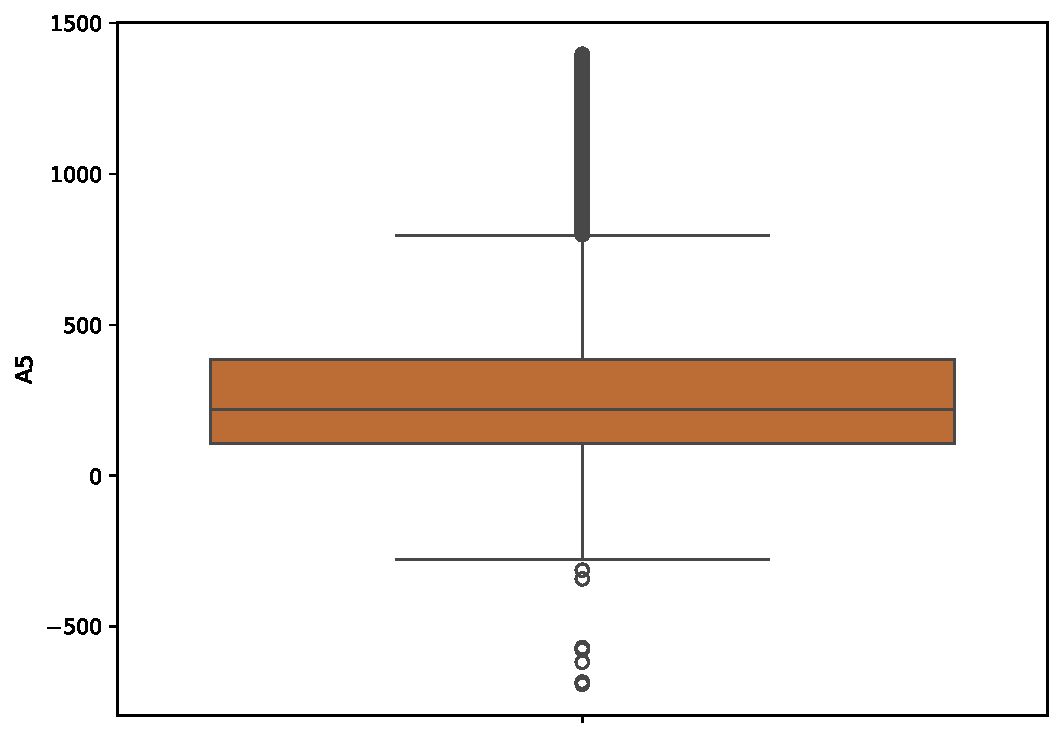
\includegraphics[width=0.6\textwidth]{images/A5_boxplot.pdf}
    \caption{Boxplot of A5.}
    \label{fig:a5_boxplot}
\end{figure}


\begin{figure}[H]
    \centering
    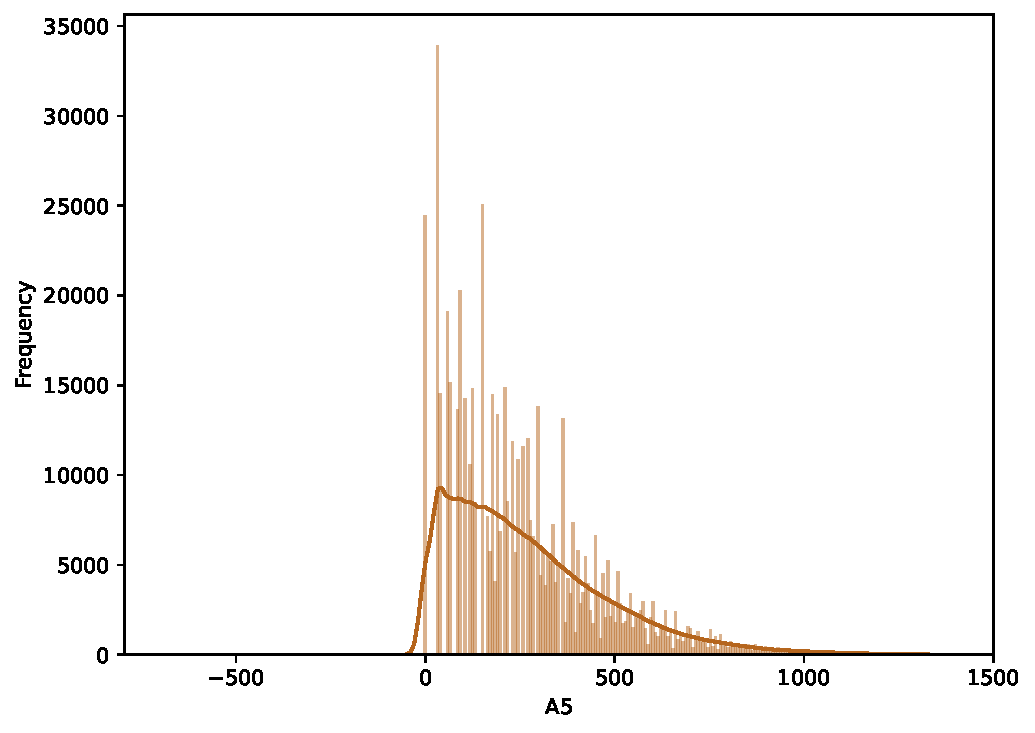
\includegraphics[width=0.6\textwidth]{images/A5_histplot.pdf}
    \caption{Histogram of A5.}
    \label{fig:a5_histplot}
\end{figure}

The boxplot in figure~\ref{fig:a5_boxplot} shows that A5 has outliers in the lower and upper range of its distribution. A5 has quite a lot of outliers on the upper end compared to only a few on the lower end. These outliers in the lower end of A5s distribution are most likely data errors, because figure~\ref{fig:a5_histplot} shows that the overwhelming majority of data is larger than zero. The fact that there are only a few negative values and they are all outliers is cause for suspicion. The outliers in the upper range of the distribution appear to be part of the normal distribution of A5.

\begin{figure}[H]
    \centering
    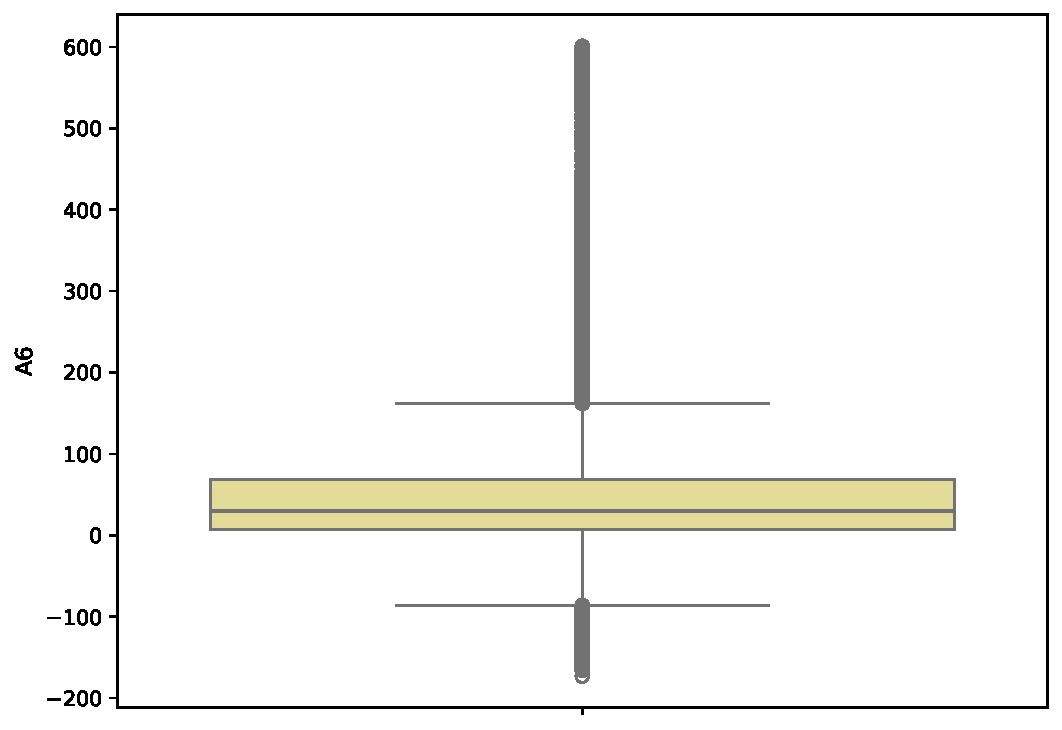
\includegraphics[width=0.6\textwidth]{images/A6_boxplot.pdf}
    \caption{Boxplot of A6.}
    \label{fig:a6_boxplot}
\end{figure}

\begin{figure}[H]
    \centering
    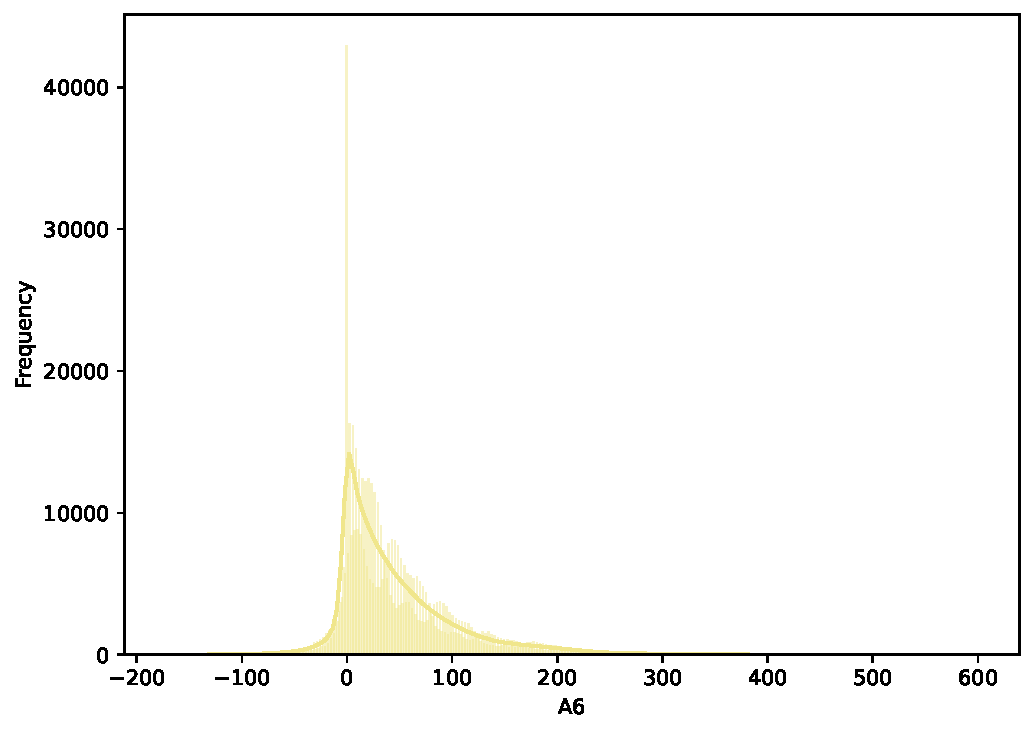
\includegraphics[width=0.6\textwidth]{images/A6_histplot.pdf}
    \caption{Histogram of A6.}
    \label{fig:a6_histplot}
\end{figure}

The boxplot in figure~\ref{fig:a6_boxplot} shows that A6 has quite a few outliers, in both the lower and upper ends of its distribution. Figure~\ref{fig:a6_histplot} shows the exact distribution of A6, and it can be seen that A6 has an extreme right-skewed distribution. These outliers form part of the natural distribution of A6 and removing them would result in a loss of information. To mitigate their influence on the machine learning model used, one could apply a transformation like the logarithmic or square root transformation. As mentioned previously this keeps the information represented by the outliers, but mitigates their influence on the fitted model.

\begin{figure}[H]
    \centering
    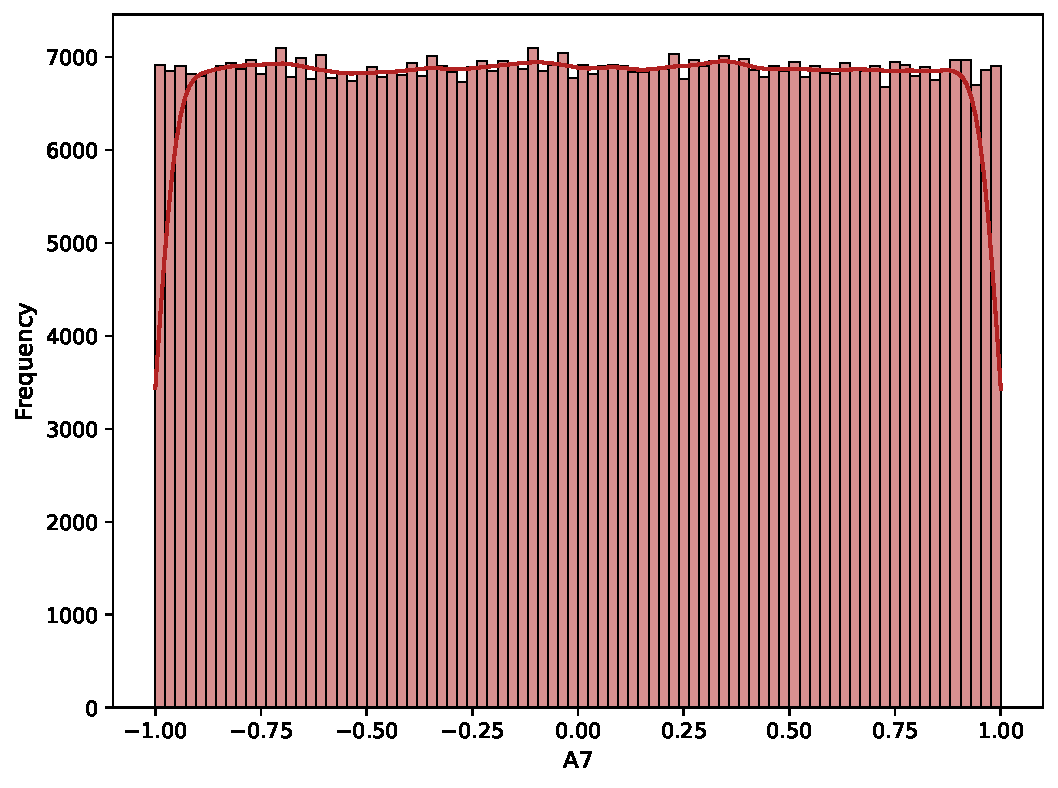
\includegraphics[width=0.6\textwidth]{images/A7_histplot.pdf}
    \caption{Histogram of A7.}
    \label{fig:a7_histplot}
\end{figure}

The histogram in figure~\ref{fig:a7_histplot} shows the distribution of A7. It indicates that A7 has an approximately uniform distribution over the range [-1, 1]. Since it also has high cardinality and a correlation of 0 with the response, feature A7 likely does not provide any useful information and including it in this dataset will likely harm any model trained on this dataset.

\begin{figure}[H]
    \centering
    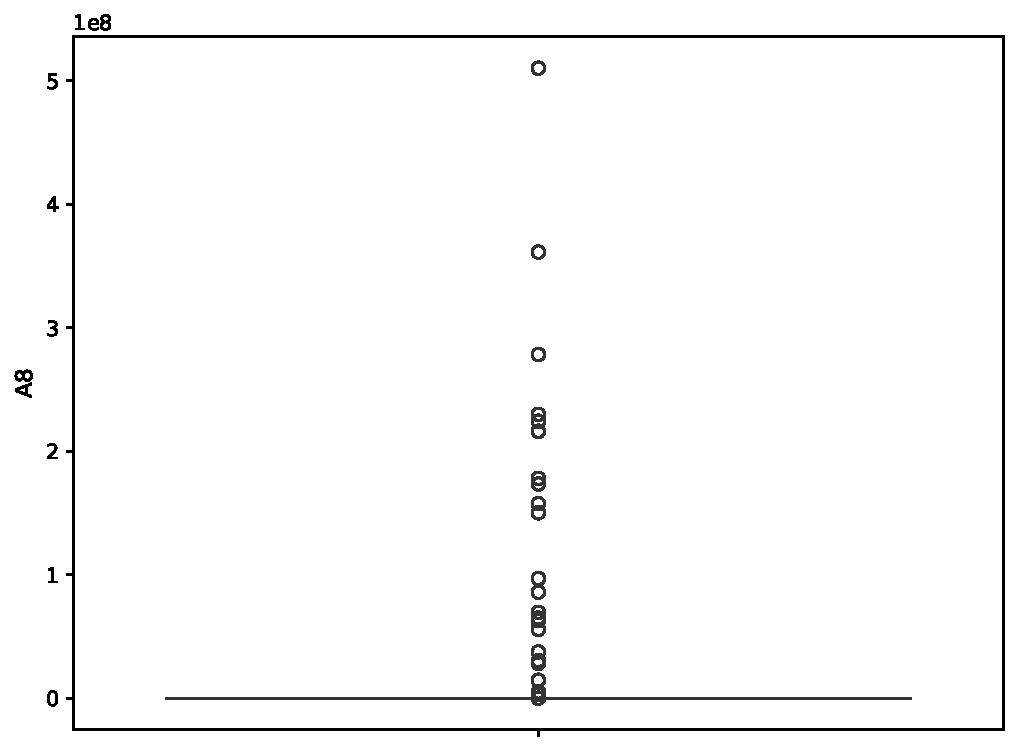
\includegraphics[width=0.6\textwidth]{images/A8_boxplot.pdf}
    \caption{Boxplot of A8.}
    \label{fig:a8_boxplot}
\end{figure}

\begin{figure}[H]
    \centering
    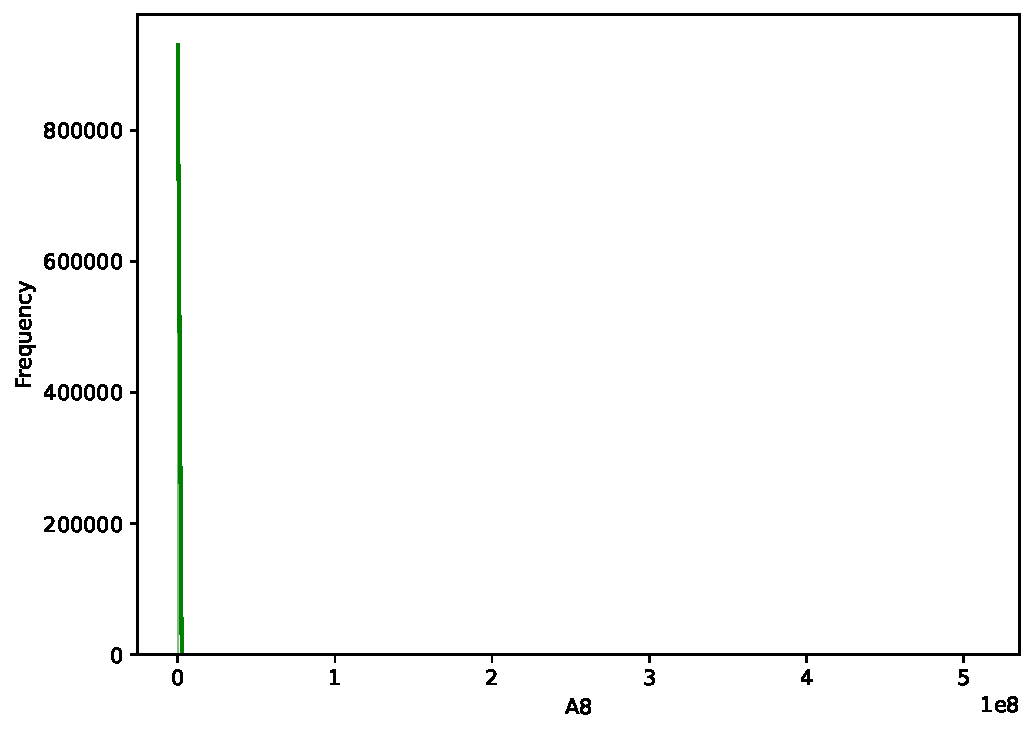
\includegraphics[width=0.6\textwidth]{images/A8_histplot.pdf}
    \caption{Histogram of A8.}
    \label{fig:a8_histplot}
\end{figure}

The boxplot in figure~\ref{fig:a8_boxplot} shows the extreme outliers in the higher end of the distribution of A8. The boxplot and the histogram in figure~\ref{fig:a8_histplot} show that these outliers cause A8 to have an extremely right skewed distribution. Although there are only a few outliers, they drastically affect the distribution of A8. They are most likely data errors since the distribution of A8 is this severely skewed and the best approach to deal with them is to remove them from the dataset.

\begin{figure}[H]
    \centering
    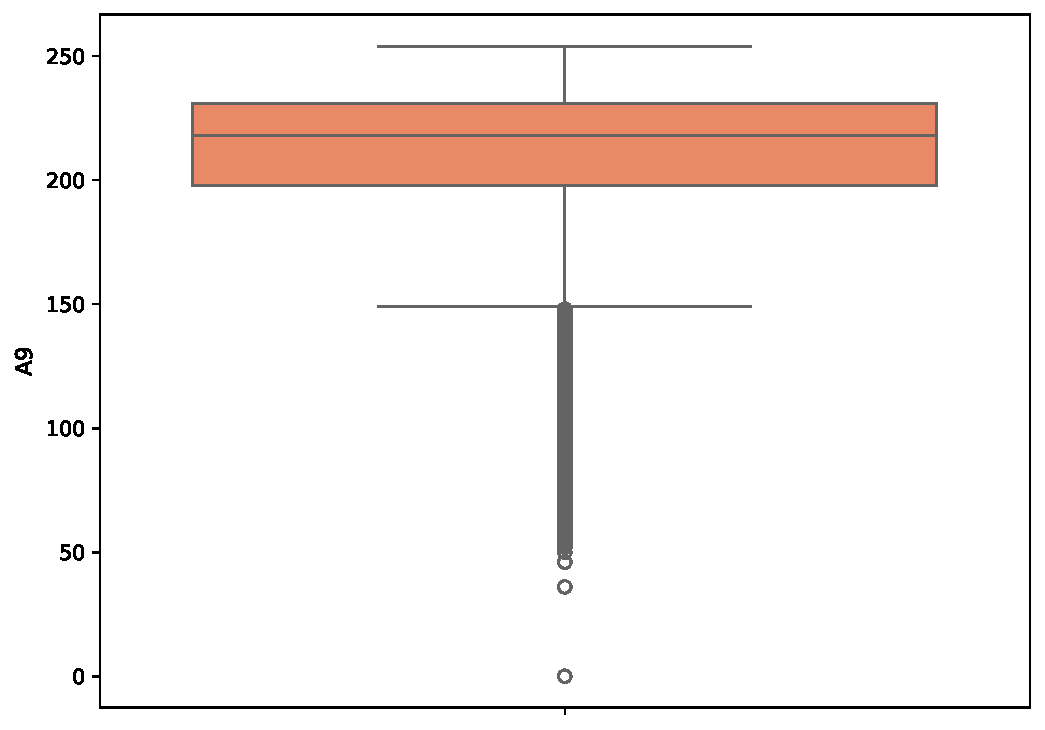
\includegraphics[width=0.6\textwidth]{images/A9_boxplot.pdf}
    \caption{Boxplot of A9.}
    \label{fig:a9_boxplot}
\end{figure}

\begin{figure}[H]
    \centering
    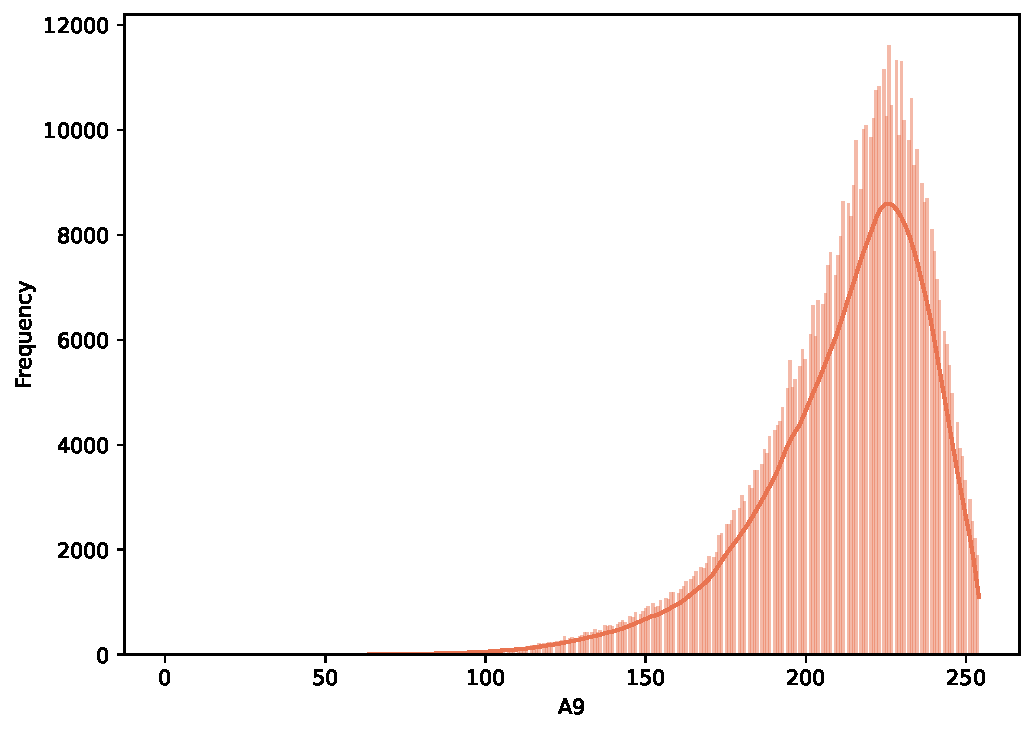
\includegraphics[width=0.6\textwidth]{images/A9_histplot.pdf}
    \caption{Histogram of A9.}
    \label{fig:a9_histplot}
\end{figure}

The boxplot in figure~\ref{fig:a9_boxplot} shows that A9 has a bunch of outliers in the lower end of its distribution. Figure~\ref{fig:a9_histplot} show that A9 has a left-skewed distribution, meaning that these outliers form part of the natural distribution of A9 and removing them would result in a loss of information. To mitigate their influence a logarithmic or square root transformation can be used, but since A9 is left-skewed, the transformation cannot be applied as is. A9 first has to be reflected to make it right-skewed and then only the transformation can be applied.

\begin{figure}[H]
    \centering
    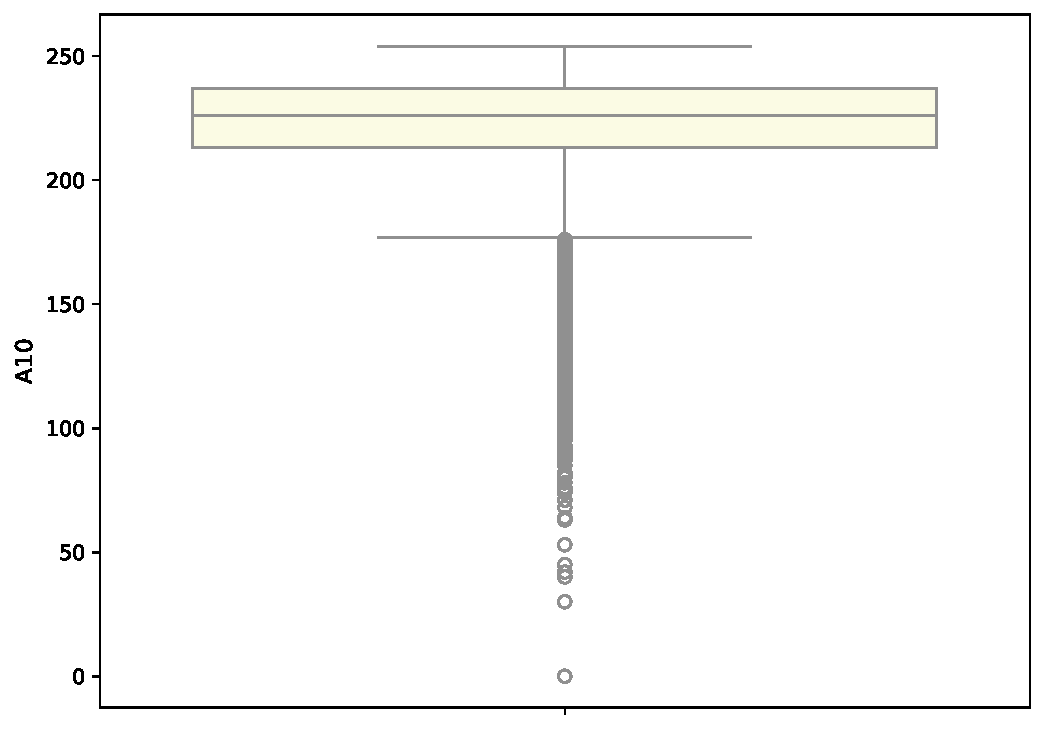
\includegraphics[width=0.6\textwidth]{images/A10_boxplot.pdf}
    \caption{Boxplot of A10.}
    \label{fig:a10_boxplot}
\end{figure}

\begin{figure}[H]
    \centering
    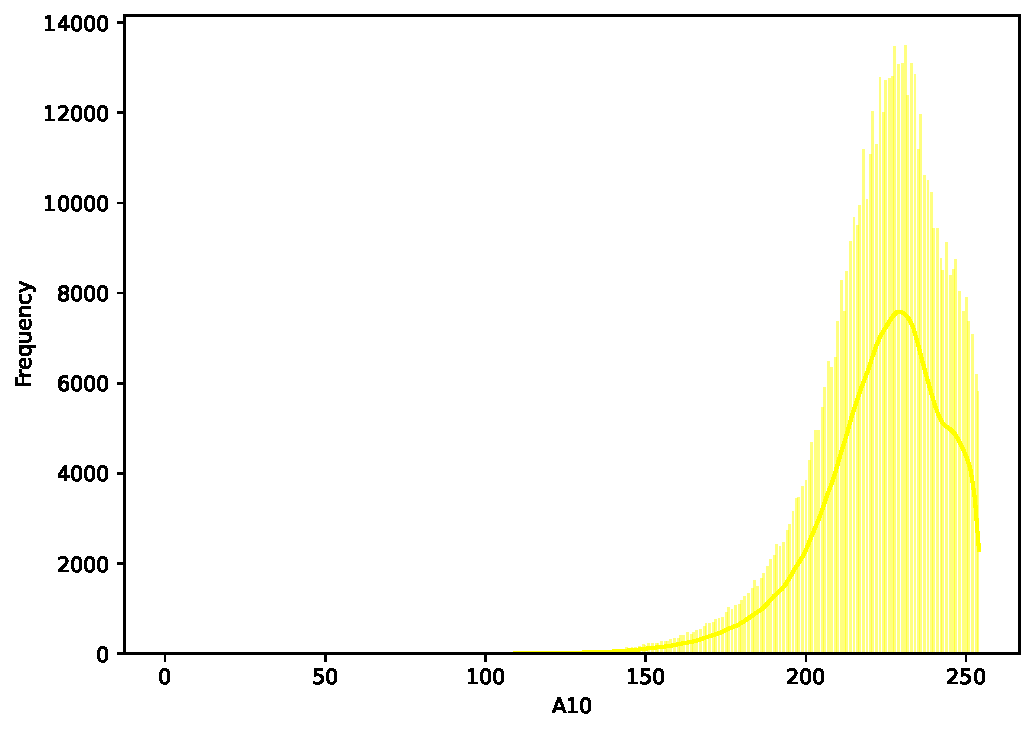
\includegraphics[width=0.6\textwidth]{images/A10_histplot.pdf}
    \caption{Histogram of A10.}
    \label{fig:a10_histplot}
\end{figure}

The boxplot in figure~\ref{fig:a10_boxplot} was drawn after preprocessing A10, and treating all instances that are not numeric, meaning all instances of \textit{a}, as missing values. This plot shows that A10 has outliers in the lower end of its distribution. Figure~\ref{fig:a10_histplot} shows that A10 has a left-skewed distribution extremely similar to that of A9, and would benefit from the same kind of transformation.

\begin{figure}[H]
    \centering
    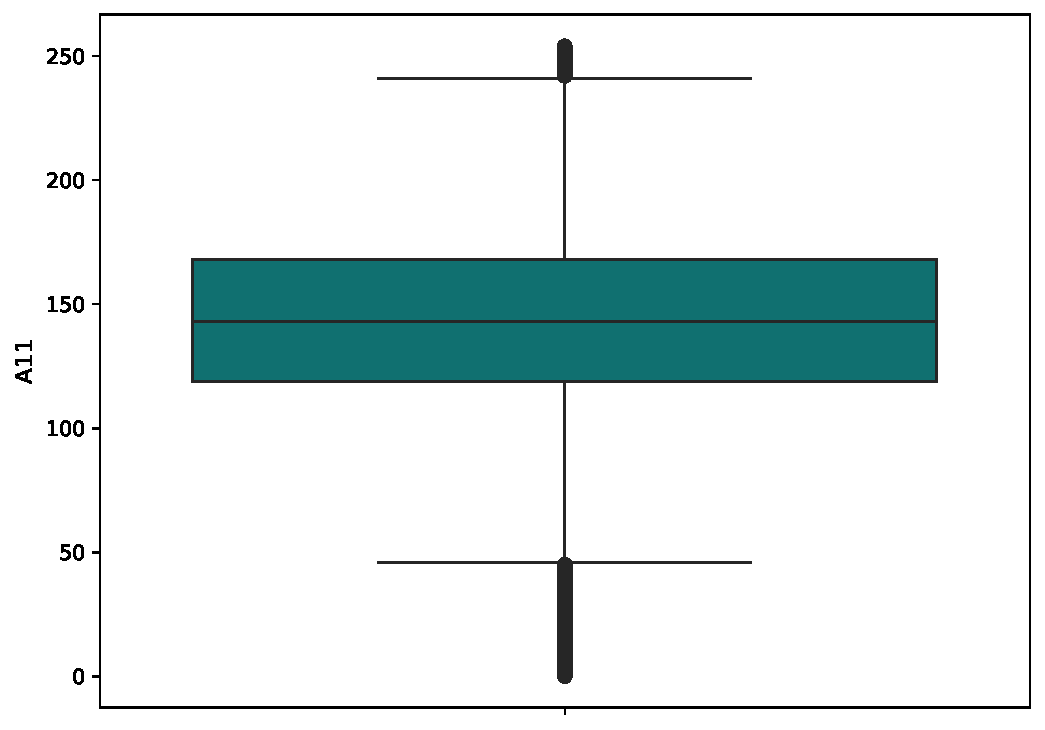
\includegraphics[width=0.6\textwidth]{images/A11_boxplot.pdf}
    \caption{Boxplot of A11.}
    \label{fig:a11_boxplot}
\end{figure}

\begin{figure}[H]
    \centering
    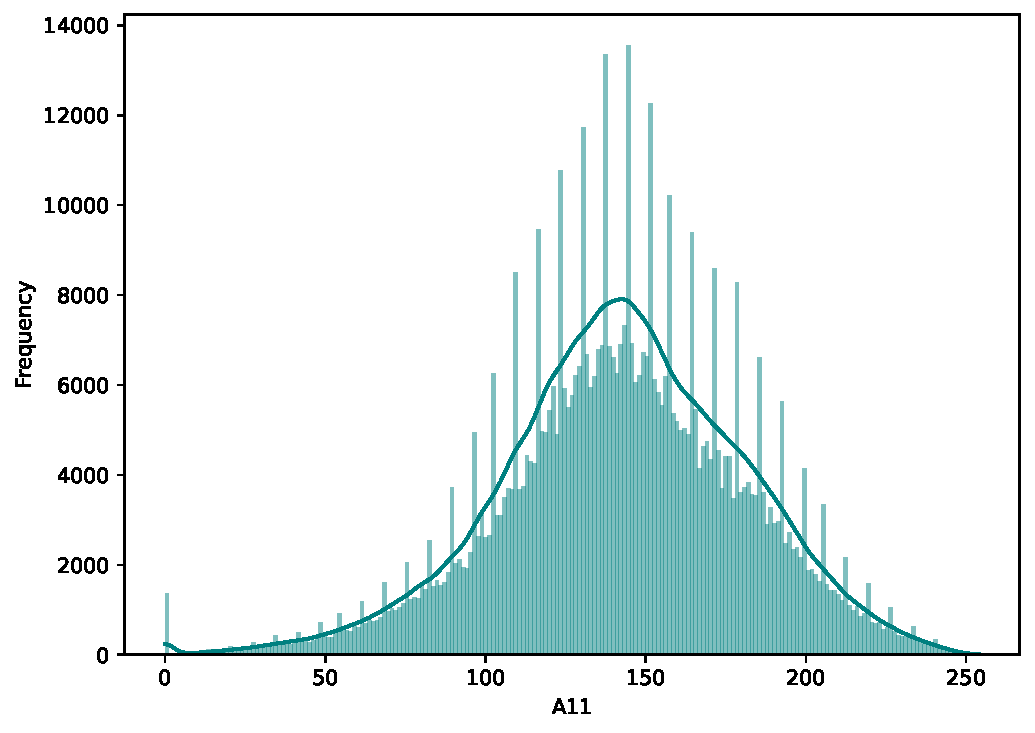
\includegraphics[width=0.6\textwidth]{images/A11_histplot.pdf}
    \caption{Histogram of A11.}
    \label{fig:a11_histplot}
\end{figure}

The boxplot in figure~\ref{fig:a11_boxplot} shows that A11 has numerous outliers in both the lower and upper ranges of its distribution. Figure~\ref{fig:a11_histplot} shows that A11 has an approximately normal distribution and the outliers in the upper and lower ranges of the distribution form part of the natural distribution of A11. Removing them would lead to a loss of information, that is why the best way to mitigate their influence on the trained model is to use a clamp transformation.

\begin{figure}[H]
    \centering
    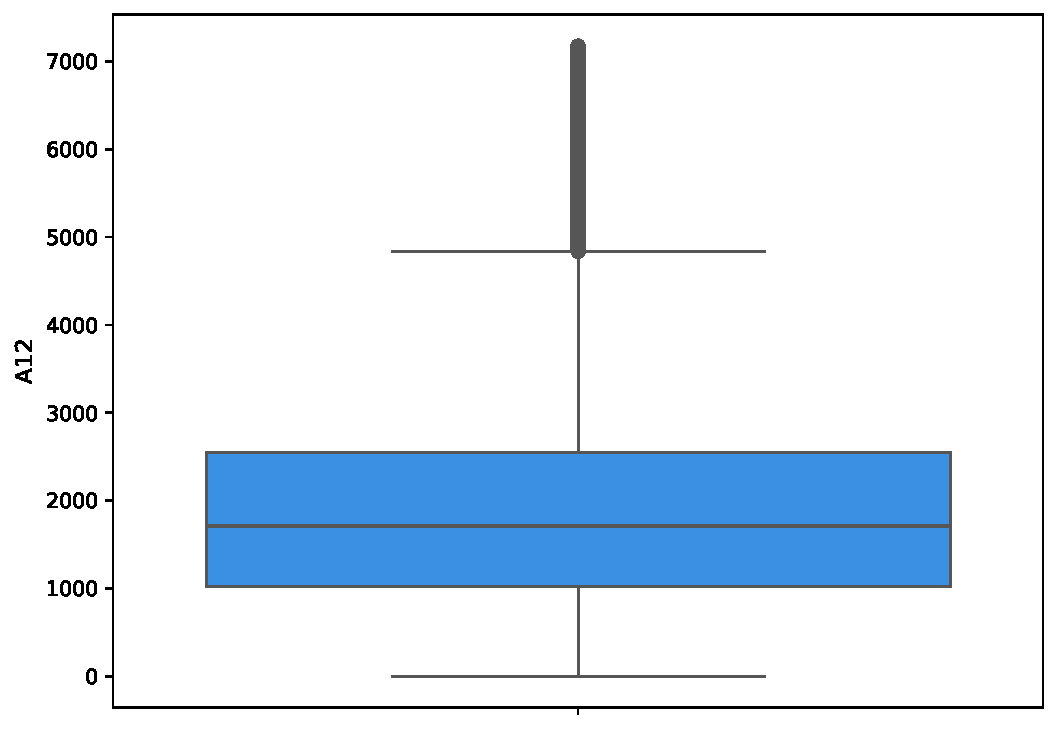
\includegraphics[width=0.6\textwidth]{images/A12_boxplot.pdf}
    \caption{Boxplot of A12.}
    \label{fig:a12_boxplot}
\end{figure}


\begin{figure}[H]
    \centering
    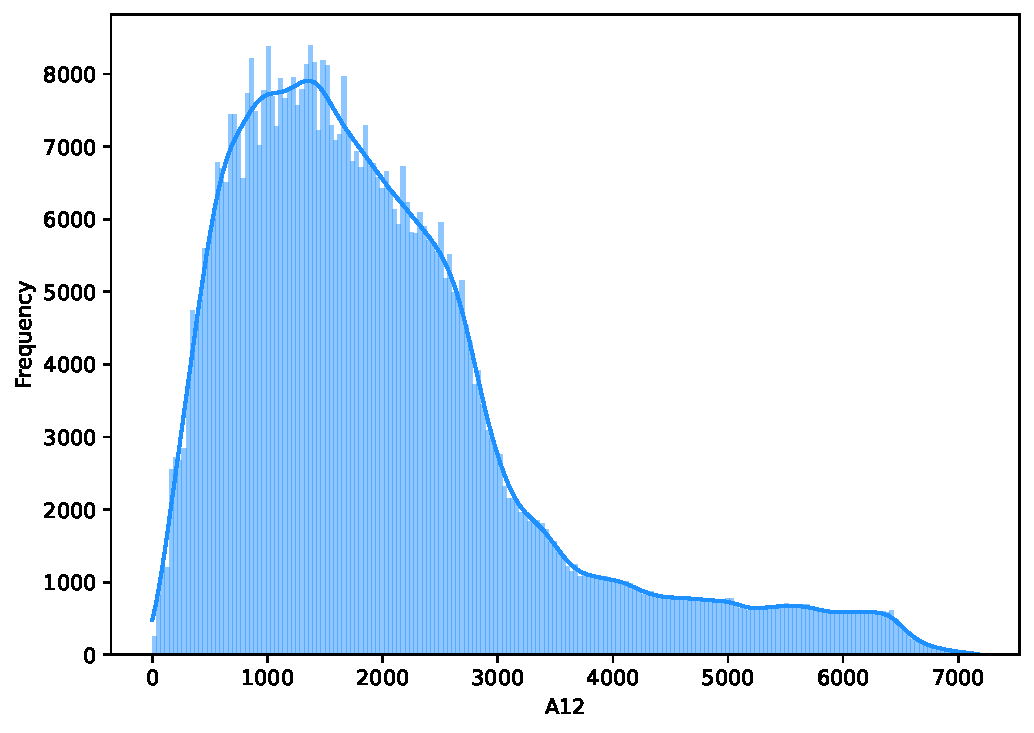
\includegraphics[width=0.6\textwidth]{images/A12_histplot.pdf}
    \caption{Histogram of A12.}
    \label{fig:a12_histplot}
\end{figure}

The boxplot in figure~\ref{fig:a12_boxplot} indicates that A12 has numerous outliers in the upper end of its distribution. Figure~\ref{fig:a12_histplot} shows the distribution of A12. These outliers in the upper range of the distribution of A12 seem to be part of the natural distribution of A12, since it is right-skewed. They are most likely not data errors and need to be kept to include the information they represent, although a transformation can be used to mitigate their influence on the trained model.

\begin{figure}[H]
    \centering
    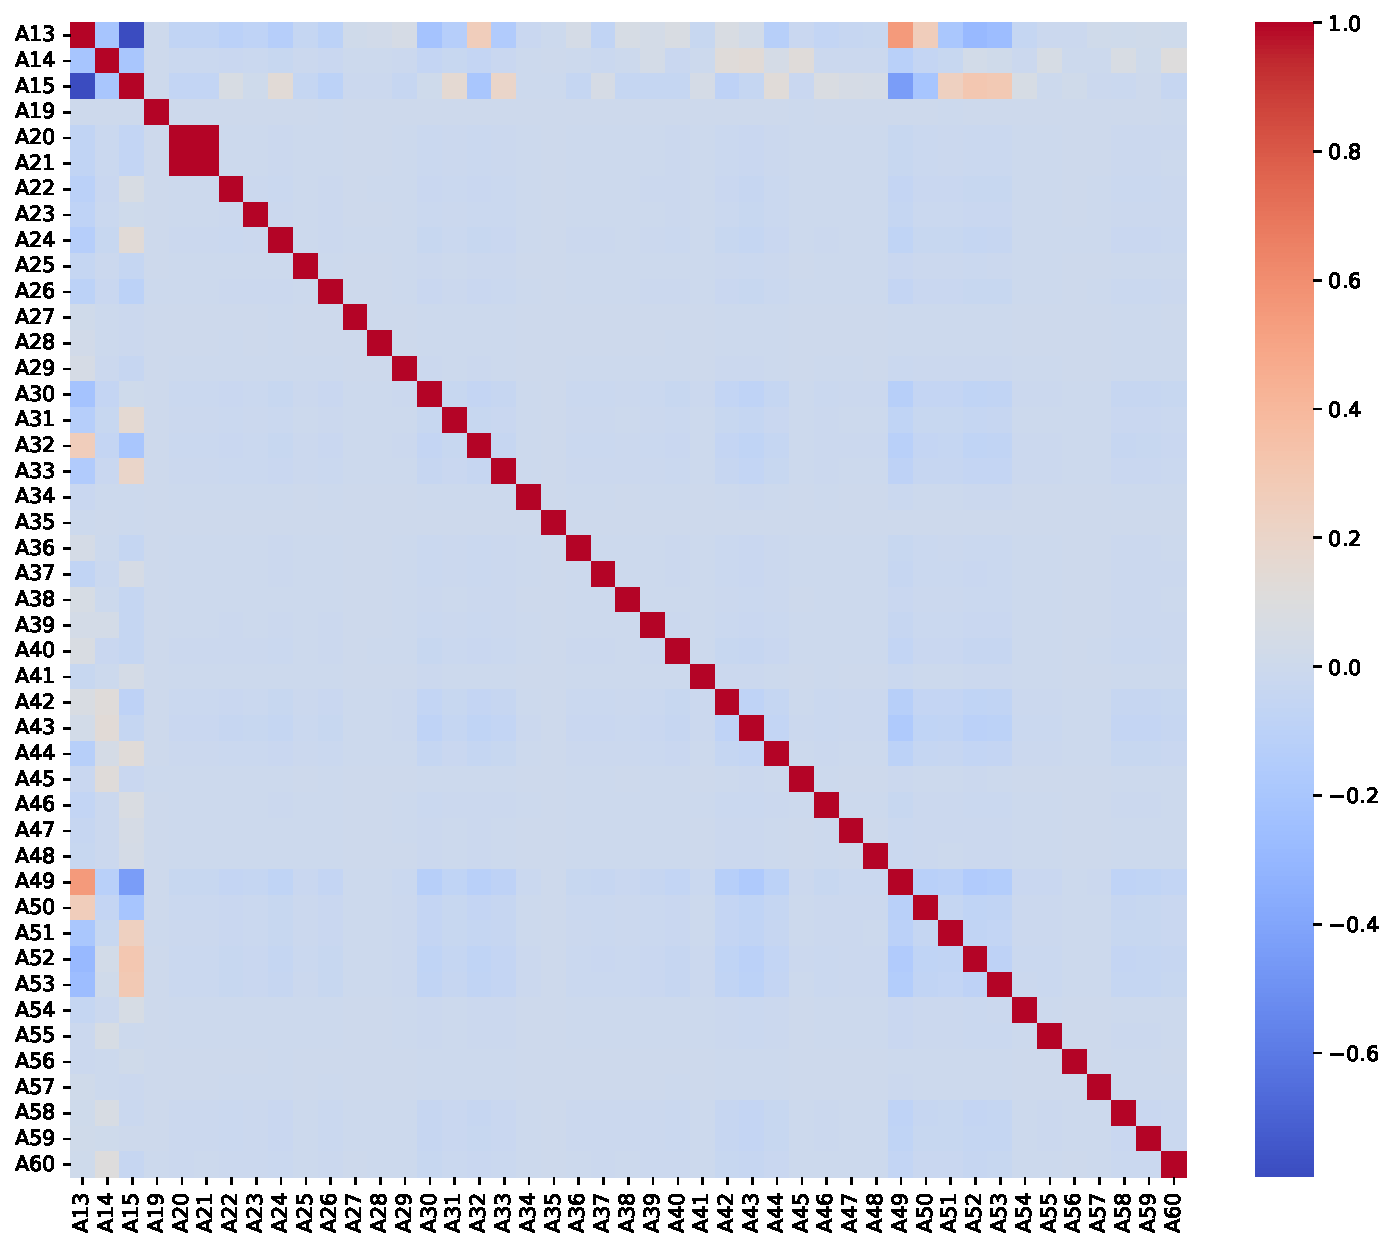
\includegraphics[width=0.7\textwidth]{images/binary_heatmap.pdf}
    \caption{Heat Map of Binary Features.}
    \label{fig:binary_heatmap}
\end{figure}

The heatmap in figure~\ref{fig:binary_heatmap} strongly suggests the presence of two groups of one-hot encoded variables. Binary one-hot encoded features created from the same original categorical variable are inherently negatively correlated. This means that distinct blocks of blue (negatively correlated) squares in the heatmap in figure~\ref{fig:binary_heatmap} correspond to encodings of a distinct original categorical variable. A13, A14, \& A15 are the first group, since they are all negatively correlated with one another. A19-A60 is another group of one-hot encoded variables as they are also negatively correlated with one another. There is correlation present between the variables in the first and second group, which also strongly suggests that these are groups of two distinct one-hot encoded categorical features.

\end{document}